\begin{refsection}

\chapter[Cortico-Amygdalar Dynamics in Taste Processing]{Coupled dynamics of stimulus-evoked gustatory cortical and basolateral amygdalar activity}

Chapter 3 is a reproduction of an article published as:\\\\
Mahmood, A., et al. “Coupled Dynamics of Stimulus-Evoked Gustatory Cortical and Basolateral Amygdalar Activity.” Journal of Neuroscience, Nov. 2022. www.jneurosci.org, https://doi.org/10.1523/JNEUROSCI.1412-22.2022.

\section{Abstract}
Gustatory cortical (GC) single-neuron taste responses reflect taste quality and palatability in successive epochs. Ensemble analyses reveal epoch-to-epoch firing rate changes in these responses to be sudden, coherent transitions. Such nonlinear dynamics suggest that GC is part of a recurrent network-that GC produces these dynamics in concert with other structures. basolateral amygdala (BLA), which is reciprocally connected to GC and central to hedonic processing, is a strong candidate partner for GC: BLA taste responses evolve on the same general “clock” as GC; furthermore, inhibition of activity in the BLA$\rightarrow$GC pathway degrades the sharpness of GC transitions. These facts motivate, but do not test, our over-arching hypothesis that BLA and GC act as a single, co-modulated network during taste processing. Here we provide just this test of simultaneous (BLA and GC) extracellular taste responses in female rats, probing the multi-regional dynamics of activity in these regions to directly test whether BLA and GC responses contain coupled dynamics. We show that BLA and GC response magnitudes covary across trials and within single responses, and that changes in BLA-GC LFP phase-coherence are epoch-specific. Such classic coherence analyses, however, obscure the most salient facet of BLA-GC coupling: sudden transitions in and out of the epoch known to be involved in driving gaping behavior happen near-simultaneously in the two regions, despite huge trial-to-trial variability in transition latencies. This novel form of inter-regional coupling, which we show is easily replicated in model networks, suggests collective processing in a distributed neural network.

\section{Introduction}
As a rat feeds, gustatory cortical (GC) single-neuron taste responses take the form of a sequence of distinct “epochs” separated by sudden ensemble transitions. The epoch that starts at 0.5-1.5sec (depending on the trial) contains firing that is staunchly palatability-related; the transition into that epoch, which is so sudden that it is analytically indistinguishable from state switching (\cite{sadacca2016a} see below for distinction of the terms “epoch” and “state”), both predicts and drives taste-related oral behavior (\cite{sadacca2012a,li2016a,mukherjee2019a}). Theory suggests that such dynamics are most easily generated by a distributed circuit in which strong recurrent connectivity (\cite{maass2007a, miller2010a, miller2013a,edelman2013a,mante2013a,kietzmann2019a}) couples “separate” regions into a single processing unit; such recurrence is abundant within the taste circuit (\cite{bielavska1996a,mcdonald1998a,shi1998a}).

Particularly notable in this regard is the reciprocally-connected GC-basolateral amygdala (BLA) dyad. Work investigating these brain regions separately (\cite{katz2001a,fontanini2009a,sadacca2012a}) has revealed striking similarities in the trial-averaged dynamics of their taste responses. Furthermore, BLA-GC connectivity has proven important for both taste learning (\cite{lin2012a,lin2015a,lavi2018a,kayyal2019a}) and taste processing (\cite{lin2021a}). This latter study specifically demonstrated that the suddenness of the behaviorally-relevant GC ensemble transitions to the palatability epoch are degraded by inhibition of BLA$\rightarrow$GC axons. These results provide indirect evidence for a general hypothesis that BLA and GC work together during taste processing, but stop far short of testing the existence of dynamic BLA-GC coupling; in fact, there has been little work directly investigating communication between any pair of taste-relevant brain regions (but see \cite{lorenzo1997a}).

Work investigating pairs of regions involved in other processes --- decision making (\cite{antzoulatos2016a,place2016a,zielinski2019a}), sensory-motor transformation (\cite{arce-mcshane2016a}), vision (\cite{bastos2015a,zandvakili2015a,saravani2019a,lundqvist2020a}), and motor planning (\cite{yates2017a,ames2019a}) --- has revealed inter-regional spiking and field potential coherence, but has done so using metrics for which temporal resolution, particularly at the single-trial level, is limited. Given the epochal nature of taste processing, the suddenness of GC ensemble transitions into palatability-responsiveness, and the trial-specific latency of this transition, testing BLA-GC coupling requires techniques that permit evaluation of the moment-to-moment evolution of the BLA-GC relationship. The fact that the suddenness of GC ensemble transitions (\cite{sadacca2016a,mukherjee2019a}) depends upon an intact BLA-GC pathway (\cite{lin2021a}) motivates our novel, central prediction: that this moment of transition will be coupled across BLA-GC ensembles. 

Here, we present an in-depth investigation of BLA-GC taste-response coordination, beginning with “canonical” methods (correlations of spiking in whole trials, and phase-coherence of local field potentials [LFP] across trials) and progressing to the testing of our novel hypothesis. The former allows us to show trial-specific and time-varying coupling in BLA and GC taste responses --- reductions in phase-coherence (\cite{stitt2017a}) that appear and vanish in an epoch-specific manner. But since these analyses necessarily obscure coupling in the trial-specific timing of sudden state-to-state ensemble transitions, we move on to explicit modeling of state transitions in ensemble timeseries data (\cite{rabiner1989a,sadacca2016a}); these analyses allow us to confirm our prediction that BLA-GC coordination integrally involves sudden, brief coupling of the specific transitions that predict and drive palatability-related behavior. Finally, computational modeling demonstrates that these results (coordinated state transitions with variable state-wise functional connectivity) are easily recapitulated within a simple multi-region network. These results overall lead us to suggest that BLA and GC form a functional “unit” for purposes of taste processing. 

\section{Materials and Methods}


\textbf{Subjects}\par
\noindent Adult, female Long-Evans rats (n = 8; 300–350g at time of electrode implantation, Charles River Laboratories) served as subjects in our study (we have observed no sex differences in the basic cortical dynamics of taste responses between male and female rats, and therefore use female Long-Evans rats because they are, in our hands, calmer than males). The rats were housed in individual cages in a temperature- and humidity-controlled environment under a 12:12 hr light:dark cycle, given ad libitum access to food and water prior to the start of experimentation, and weighed daily following surgery to ensure that they never dropped below 80\% of their pre-surgery weight. All experimental methods were in compliance with National Institutes of Health guidelines and were approved in advance by the Brandeis University Institutional Animal Care and Use Committee.

\smallskip
\noindent\textbf{Electrode and intra-oral cannula construction}\par
\noindent Custom microwire bundle drives were made with either 16 or 32 electrodes per recording site (design and construction details available at \url{https://katzlab.squarespace.com/technology}). Intra-oral cannulae --- flexible tubing with a flanged tip and washer to ensure stability, connected to a plastic top complete with a locking mechanism --- were built to allow the delivery of tastants directly onto the tongue (\cite{fontanini2006a}).

\smallskip
\noindent\textbf{Acquisition of electrophysiological data }\par
\noindent Electrophysiological signals from the micro-electrodes were sampled at 30 kHz using 32-channel analog-to-digital converter chips (RHD2132) from Intan Technologies, digitized online at the head stage and sampled jointly, along with signals from actuators marking tastant delivery, using an Intan RHD USB interface board (Part \#C3100), which routed records to the hard drive of a PC for saving. The experimental chamber was ensconced in a Faraday cage that shielded recordings from external electromagnetic influences.

\smallskip
\noindent\textbf{Surgery}\par
\noindent Rats were anaesthetized with an intraperitoneal injection of ketamine/xylazine cocktail (100mg/kg and 5.2 mg/kg respectively) and mounted in a stereotaxic instrument (David Kopf Instruments; Tujunga, CA) with blunt (atraumatic) ear bars. A midline incision exposed the skull and trephine holes (approx. 2 mm diameter) were drilled above BLA and GC. For 6 (out of 8) rats, microwire bundles were implanted 0.5mm above GC (coordinates: AP +1.4 mm, ML -5.0 mm, DV -4.4mm from dura) and BLA (coordinates : AP -3.0mm, ML -5.0mm, DV -6.8mm from dura). For the remaining 2 rats, bundles were instead implanted bilaterally above BLA. Once in place, electrode bundles were cemented to the skull. Once electrode bundles were secured, an intra-oral cannula (IOC) was threaded through the masseter muscle (inside the zygomatic arch) to the space between the lip and gums, and the top of the cannula was cemented to the rest of the assembly with dental acrylic (\cite{fontanini2006a}). The rat’s body temperature was monitored and maintained at approx. 37°C by a heating pad throughout the duration of the surgery.

\smallskip
\noindent\textbf{Habituation and passive taste administration}\par
\noindent Following their recovery from surgery, we habituated rats to the experimental chamber for 2 days, to the IOC/electrode harness for the next 2 days, and to passive water deliveries for the following 2 days, before beginning data collection. Starting with the second habituation day, we also placed rats on a mild water restriction schedule --- 20mL of water (not including the approx. 4mL delivered during habituation sessions themselves) per day. This water restriction schedule was maintained till the end of the experiment. For the 2 final habituation sessions, we attached the rats to the taste delivery apparatus, and infused 120 pulses of distilled water (approx. 30$\mu$L per pulse; 20s inter-pulse interval) into the animal’s oral cavity through the IOC, and drove electrode bundles deeper (by 250 $\mu$m) into target structures. By the end of this procedure, the tips of the electrodes lay within GC and BLA. We then recorded taste responses during 3-4 days of taste delivery sessions, between each of which the microwire bundle was driven down approximately 60 $\mu$m. During these sessions, Sucrose (0.3M), Sodium Chloride (0.1M), Citric Acid (0.1M), and Quinine (1mM), dissolved in ultra-pure water (approx. 30$\mu$L per pulse; 20s inter-pulse interval, 30 trials/tastant) were delivered to passive rats (i.e., no behavior was required to elicit delivery). These concentrations were chosen to represent a range of hedonic values, and because they are known to evoke robust responses in both GC and BLA (\cite{fontanini2009a,sadacca2012a}).

\smallskip
\noindent\textbf{Histology}\par
\noindent In preparation for histology, rats were deeply anesthetized with an overdose of the ketamine/xylazine mixture. We perfused the rats through the heart with 0.9\% saline followed by 10\% formalin and harvested the brain. The brain tissue was incubated in a fixing mixture of 30\% sucrose and 10\% formalin for 7 days before being sectioned into 50$\mu$m coronal slices on a sliding microtome (Leica SM2010R, Leica Microsystems). Sections containing the electrode implant sites around GC and BLA were imaged at 2x.

\smallskip
\noindent\textbf{Data and statistical analyses}\par
\noindent The analysis of data and statistical tests were performed using custom written software in Python and MATLAB (The MathWorks, R2018a), as described below.

\smallskip
\noindent\textbf{Local Field Potential processing and analysis}\par

\noindent\underline{Filtering / power and phase extractions}
LFPs were extracted from broadband digitized signals using a 2nd order bandpass Butterworth filter (1-300Hz), to de-emphasize spiking and emphasize frequencies typically of interest in such data. In order to avoid contamination from noise/artifacts on noisy/broken channels, only channels containing isolable single neurons (see below) were used for analyses. Estimates of instantaneous power and phase in delta (1-4Hz), theta (4-7Hz), mu (8-12Hz), beta (12-30Hz), gamma (30-100Hz) bands were extracting using the Short Time Fourier Transform (STFT) implementation in Scipy (\cite{p2020a}) with a 500ms window and 99\% window overlap.

\smallskip
\noindent\underline{LFP Phase Coherence}
Phase coherence analysis was performed, as per \cite{kramer2020a}, to provide a basic, dynamic, trial-averaged evaluation coupling of BLA and GC as visible in LFPs. We selected for this analysis the electrodes from which activity was most similar to the mean activity for the region (smallest mean-squared error relative to the mean phase across all channels for each region; this selection of channels was constant for all trials in a single analyzed session, and the same set of channels was used for all frequencies), to ensure reliable representation of each. The difference in phase between the (GC and BLA) pair of electrodes for each timepoint was calculated across all trials, and the mean of those phase-difference vectors was calculated for each timepoint, the magnitude of which represents the coherence strength.  Coherence values were averaged across small canonically-defined frequency bands: theta (4-7Hz) and mu (8-12Hz). Results in other bands were comparable (see Results). The specific calculation was as follows:

$$\text{Coherence}_{\text{GC}\leftrightarrow\text{BLA}}(f)=\abs{\frac{1}{N}\sum_{n=1}^{N}e^{-i(\theta_t^\text{GC}(f)-\theta_t^\text{BLA}(f)}}$$
\noindent Where $\theta_t^\text{GC}(f)$ and $\theta_t^\text{BLA}(f)$ are the GC and BLA LFP phases for time “t” and frequency “f”, and “n” is the counter for number of trials.

The error term for the evaluation of coherence magnitude was estimated using bootstrapping, by resampling trials with replacement from individual recordings (500 such resamples were performed for each recording). Changes in taste-induced coherence were determined relative to baseline (the 750 to 250ms period prior to stimulus delivery was selected as baseline, with timepoints closer to stimulus delivery ignored to avoid temporal “bleed” of coherence between pre- and post-stimulus periods due the slow frequencies considered here); if the mean value of the coherence during taste responses fell outside the 95\% CI of the baseline period (see above), the deviation was deemed significant. The fraction of recordings with significant deviations were summed at each timepoint and across all recordings, enabling an estimation of the aggregate dynamics of these changes, and the resultant time-series were smoothed (to remove brief, spurious deflections) using a 2nd order Savitzky-Golay filter with a 101 ms kernel (Press and Teukolsky, 1990). To visualize the dynamics of this phase coherence, changes in coherence from baseline were calculated for 4-7, 7-12, 12-30, 30-70, and 70-100Hz, smoothed as above, and projected into 3-dimensional space using Principal Component Analysis implemented in scikit-learn (\cite{pedregosa2011a}).

A trial-shuffled control was used to test whether calculated phase coherence reflected a default similarity in BLA and GC LFP – i.e., to test whether there were similarities between the regions on single trials above and beyond those visible in trial-averaged presentations. Essentially, the same phase-coherence calculations as above were performed on data for which trial order was shuffled between the pair of channels being compared. Differences between datasets (inter-region, intra-region, and shuffle) were then evaluated using the Repeated Measures ANOVA implemented in Pingouin (\cite{vallat2018a}), with Comparison Type and Frequency Band as factors, followed by pairwise Mann-Whitney U Tests for post-hoc analysis.

\noindent\textbf{Analysis of Spiking Activity}\par
\smallskip

\noindent\underline{Single Unit Isolation}
Spikes from electrophysiological recordings were sorted and analyzed off-line using in-house Python scripts (\url{https://github.com/abuzarmahmood/blech_clust}). Putative single-neuron waveforms with \(>\)3:1 signal-to-noise ratio were sorted using a semi-supervised algorithm: recorded voltage data were filtered between 300-3000Hz, grouped into potential clusters by a Gaussian Mixture Models (GMM) fit to multiple waveform features; clusters were then labeled and/or refined manually (to increase conservatism) by the experimenters (for details see \cite{mukherjee2017a}). 

\noindent\underline{Evaluating single-neuron response taste specificity. }
To statistically determine the degree to which a single neuron’s response contained taste-specific information, firing rates were estimated by binning spikes using rectangular rolling windows (length: 250ms, step: 25ms). A one-way ANOVA (between tastes) was then run on each window to identify if the response of a single neuron to one taste was different from its responses to any other tastes at that timepoint; as the ANOVA was run separately for each time-bin and trials of different “conditions” (i.e., tastes) were separated by tens of seconds and randomized in order, the assumption of data independence (to which the analysis is fairly robust) was not inappropriately held. To lessen the likelihood of misidentifying random noise from true responses, a time-bin was deemed to have significantly discriminative responses if it was part of 3 consecutive time-bins with a p-value \(<\) 0.05.

\noindent\underline{Evaluating single-neuron response palatability-relatedness.} To statistically determine the degree to which a single neuron’s response reflected the hedonic value of the stimuli delivered, we smoothed firing rates as described above, and calculated the Pearson’s correlation coefficient between the evoked firing rates and the palatability ranks of the tastants. Palatability ranks  ---  sucrose (1) \(>\) NaCl (2) \(>\) citric acid (3) \(>\) quinine (4)  ---  directly reflected consumption of (earlier-run squads of) rats in a Brief Access Task (see \cite{sadacca2012a}). This ordering is canonical, and has been replicated in many studies and with multiple measures of stimulus appreciation (\cite{travers1986a,clarke1998a,fontanini2006a}). Again, we reduced the likelihood of spurious positives in the noisy time series of neural firing by deeming neural responses to be significantly correlated with palatability only if the calculated r value reached a p-value of \(<\) 0.05 for 3 consecutive time-bins.

\noindent\underline{BLA-GC Spike Count Correlation}
We extracted paired time-series of spike counts across the 0-2000 ms post-stimulus delivery for each trial. First-order differencing was performed on these timeseries to mitigate effects of serial correlations, after which the data were standardized using Z-scoring. Correlations between the spike trains, and corresponding p-values, were calculated using Scipy’s implementation of Spearman’s Rho (\cite{p2020a}). To aggregate comparisons within a single recording, the fraction of correlations achieving significance across all combinations of inter-region neuron pairs (for a single recording session) was calculated. As a control, this same fraction of significant correlations was calculated for 4000 trial-shuffled comparisons for each dataset, to generate bounds on the fraction of significant correlations expected by chance. If the value for fraction of significant correlations present in the actual data was beyond the 95\% percentile for the corresponding shuffle distribution, the value was deemed significant. 

\noindent\textbf{Changepoint Modeling of Population Activity}\par
\smallskip

\begin{figure}
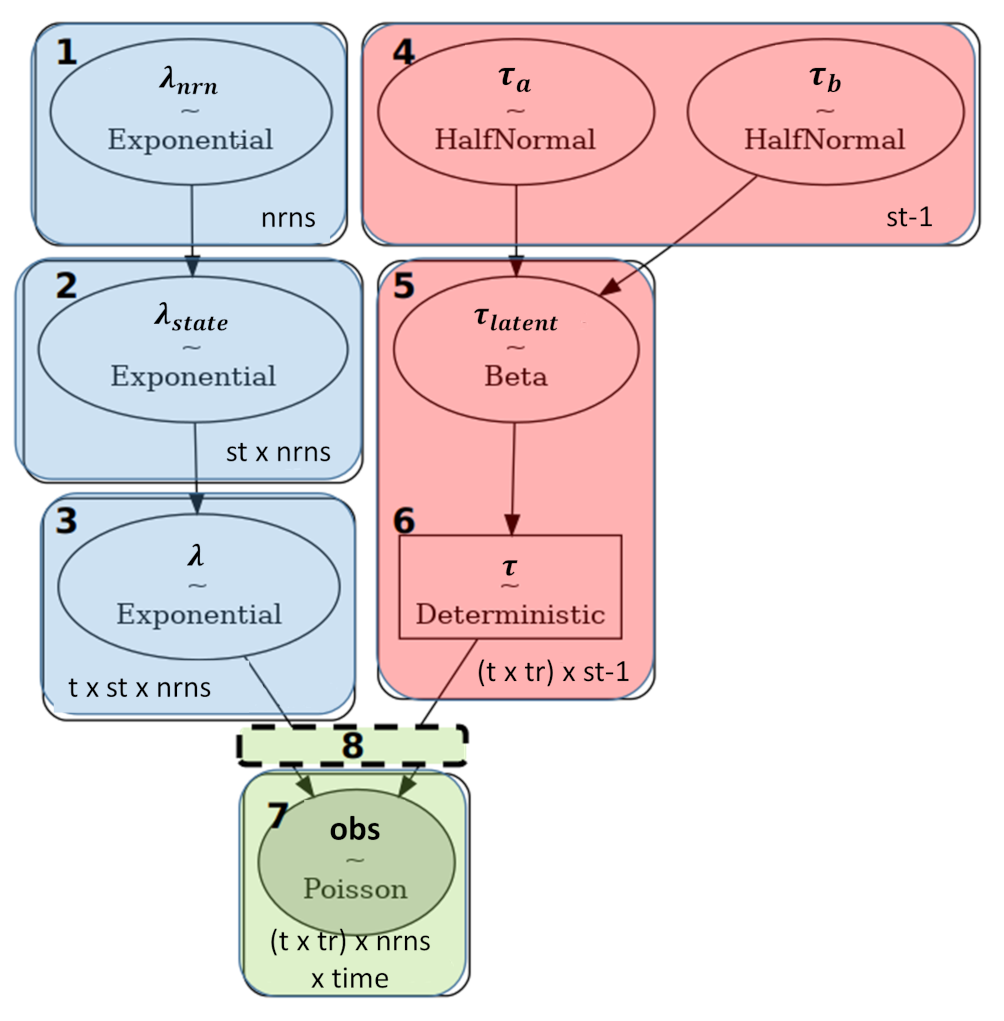
\includegraphics[width=\linewidth]{mahmood_22_figures/fig1-0.png}
\caption{\textbf{Dependencies between the random variables for constructing the changepoint model.} Different colors denote different parts of the model: Blue = Emission Variables, Red =Changepoint Position Variables, Green = Likelihood. Numbers on top left of each module (rectangle) correspond to the variable (equation) each module represents. Numbers on bottom right of each module correspond to the shape of the variables (and match with the shapes defined in the equations above). nrns = neurons, st = states, t = tastes, tr = trials, time = time bins}
\label{fig:wrapfig}
\end{figure}

\noindent\underline{Model fitting for GC.} GC ensemble taste responses have been repeatedly shown to involve sudden, coherent firing rate transitions. Because these transitions typically involve firing rate changes in approx. 50\% of the neurons in simultaneously recorded ensembles (\cite{jones2007a}), and because they are sudden and stark (see below), they can be observed in single trials using any of a number of methods (see \cite{mukherjee2019a}) and can be robustly inferred from ensembles as small as six neurons (\cite{jones2007a}). Here, a multi-changepoint model written in the probabilistic programming language pymc3 (\cite{salvatier2016a}) was used to determine the presence and latency of changes in ensemble responses.

It is important to note the uncertainty inherent in measuring the latency (and hence duration) of these transitions between hidden states using point process data (spike trains). This uncertainty is a function of the magnitude of firing rate changes, the noisiness of the spike trains themselves, and the number of simultaneously recorded neurons. Taking these constraints into account, previous work has shown (\cite{sadacca2016a}) that the durations of transitions in recorded data are statistically indistinguishable from those observed using simulated data for which the underlying transition was by design instantaneous–i.e., for which the firing rates of simulated spike trains changed instantaneously at state transitions (note that the latency of these transitions were taken from analysis of experimental data, and therefore the simulations generated spike trains with PSTHs identical to those in the real data). Such analyses allow us to confidently conclude that the transitions detected in actual data (though they might appear longer due to noisy inference) likely correspond to instantaneous changes in the underlying firing rates of the neurons.

A detailed explanation of the change-point model structure and code used to identify ensemble transition times can be found online \href{https://github.com/abuzarmahmood/pytau/blob/development/pytau/examples/Bayesian_Changepoint_Model.ipynb}{(GitHub)}. Briefly, taste-evoked spike trains (the 2000ms after stimulus delivery) were binned into 50ms bins. Poisson likelihood was used to model the binned spike counts. The model is broken down, in a manner similar to a Hidden Markov Model, into two sets of latent variables: 1) the emission variables (i.e. firing rates), and 2) the changepoint position variables (i.e. when changepoints occur). 

\begin{figure}
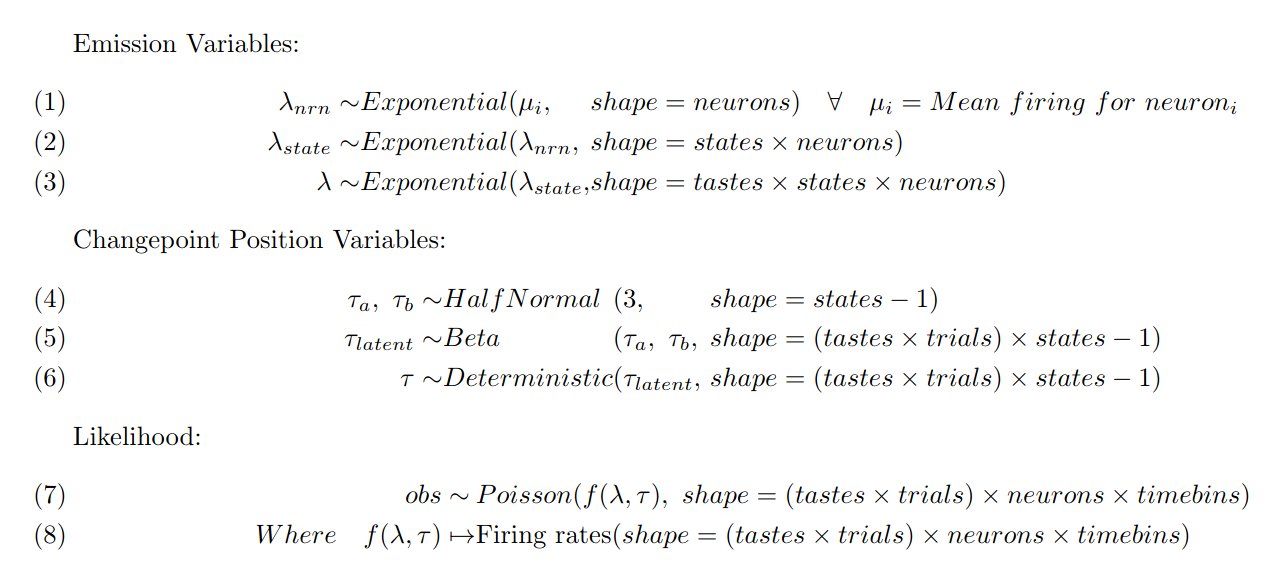
\includegraphics[width=\linewidth]{mahmood_22_figures/mahmood_changepoint_equations.png}
\end{figure}

A single-neuron’s response to different tastes will be more similar than the responses of different neurons (even to the same taste). Equations 1-3 below hierarchically model firing rates (emissions) to exploit this similarity, such that the mean activity of each neuron is modelled independently $\lambda_\text{nrn}$, Eq. 1),emissions for each state and neuron $\lambda_\text{state}$ are dependent on $\lambda_\text{nrn}$ (Eq. 2), and emissions for each taste, state, and neuron $\lambda$ are dependent on $\lambda_\text{state}$ (Eq. 3). This results in values of $\lambda$ being drawn from a distribution of $\lambda_\text{state}$ values, which in turn are drawn from distributions of $\lambda_\text{nrn}$ values. This organization better constrains the space of emission values during different states for each neuron (i.e. the model knows the emission for State 1 for Neuron 1 will be similar to State 2 for the same neuron), allowing the model to fit more robustly. Equations 4-6 model the changepoint positions, assuming that the distribution of hyperparameters $\tau\text{_a}, \tau\text{_b}$ for a changepoint are shared across all trials for each given changepoint (e.g. hyperparameters for first transition is shared for the first transition across all trials, likewise the second transition, etc), but different for different changepoints. Finally, the latent emissions and changepoints are combined to generate timeseries of firing rates with sequential states (Eq. 8 is a deterministic function, refer to URL above for exact implementation), which is used to evaluate the likelihood of the data given the latent variables (Eq. 7). The dependencies between the equations are visualized in Fig. 3.1 below.
 
A modularized pipeline was used to fit and analyze the models across datasets (\href{https://github.com/abuzarmahmood/pytau/tree/development/pytau}{PyTau-GitHub}).

\noindent\underline{Model fitting for BLA.} The same changepoint analyses described above were also brought to bear on BLA ensembles, to test whether BLA population dynamics can be validly described, like those observed in GC, as transitioning suddenly and coherently. For these analyses, we used a separate cohort of 2 rats (9 recording sessions in total) in which we performed bilateral BLA recordings to obtain larger neural populations (results were qualitatively similar for those obtained from BLA-GC dual-region recordings). 

We compared goodness-of-fit for changepoint models fit to the recorded (actual) data with that for models fit to two surrogate datasets in which the single-trial coordination of the neural population was perturbed. To generate these surrogate datasets, we started with the actual observed spike train data, and either 1) randomly shuffled whole trials for single neurons (e.g., such that Trial 1 for one neuron was paired with Trial 4 for another neuron), or 2) shuffled individual spikes from one trial to the same time-bin in another trial for the same neuron. Both of these shuffling processes create datasets for which single-neuron PSTHs remain identical to the original, while disrupting any coherent changes in population activity present on single trials (see Fig. 3.4A).  

Model fitting was performed using Automatic Differentiation Variational Inference (ADVI, \cite{kucukelbir2016a}) capabilities present in pymc3. The ADVI algorithm optimizes the Evidence Lower BOund (ELBO) of the model. The ELBO is a lower limit on the marginal likelihood of the model (\cite{blei2017a}); it automatically penalizes more complex models (which necessarily provide better apparent fits because they have more free parameters), allowing for model comparisons similar to the various Information Criteria. The ELBO is an integral part of the model fitting procedure, which makes it convenient and efficient to use as a tool for performing model comparisons. Statistical significance of differences between ELBO values for the actual data and shuffle conditions were determined using the 2-Way Repeated Measures ANOVA (from Pingouin) with Model States and Shuffle Type as factors.

\noindent\underline{Determining number of states}. Since a timeseries can be fit with a model containing an arbitrary number of states, we performed model comparison to determine the most parsimonious number of states to describe BLA taste ensemble activity (0-2000 ms post-stimulus delivery). We fit models with 2-10 states to each BLA population and used the ELBO for model comparison.  For each dataset, we ranked the different models using their respective ELBOs. 

\noindent\underline{Transition-aligned changes in recorded activity vs. “smooth” surrogate data.} To supplement the above comparisons (and thereby further test and/or strengthen our conclusions), we compared the magnitude of firing rate changes across inferred changepoints in the actual data to that in the two above-described surrogate datasets. Given that these magnitude changes should be maximal only when changepoints are correctly identified at the ensemble level-i.e., when all neurons in the ensemble change their rates simultaneously in the trial-we would expect that changes in both single-neuron and population activity would be greater across inferred changepoints for the actual data vs the shuffled datasets. After inferring changepoints for models with 4 states (this number of states was determined to provide the best fit to our data; see Fig. 3.4), we computed the average firing rate in 500 ms bins on either side of each changepoint, calculating the magnitude of change across the changepoint for both single neurons and of the whole neural population (analyzed as changes in an instantaneous-activity vector comprised of all simultanteously-recorded neurons in a session). To compare both the average magnitude and pervasiveness of differences between activity in the datasets (to enhance conservativeness by accounting for the few large outliers skewing average changes in magnitude), we calculated: 1) The number of neurons for which, on average, the actual data had larger magnitude of change across the transitions; 2) the number of neural populations for which the actual data had a larger magnitude of change across the transition; 3) the fold-change of magnitude in firing for single neurons (shuffled data/actual data); and 4) the fold change in magnitude of the population vector. The number of larger neural transitions was calculated by assessing which group (actual data, whole-trial shuffle, spike-trial shuffle) had the largest change in activity across the transition, for every transition; this produces ratios for which group he largest transition belonged to.

Testing for significance of the likelihood that transitions  are larger in the recorded data than in control simulations (points 1 and 2 above) was carried out using a One-Way ANOVA followed by Tukey’s post-hoc test. Hypothesis testing for differences in magnitude was performed using Wilcoxon signed-rank test with Bonferroni’s correction (points 3 and 4 above). 

\smallskip
\noindent\textbf{Coordination of BLA and GC Transition Times}\par
\noindent To test our central hypothesis regarding the coupling of BLA and GC transitions in single trials, we assessed synchronization of transition times using simple correlative statistics.

\noindent\underline{Testing transition-time correlation as a coordination metric.} To test the utility of this approach, we first performed pilot analyses on GC ensembles (which are known to transition suddenly) with higher counts of simultaneously recorded neurons (n$\ge$10neurons/population). We divided these ensembles into two populations randomly, repeating the splits 10 times/ensemble to avoid any issues related to selection of unrepresentative groups. Transition times were inferred independently for each half-ensemble (using techniques described above), after which the values for transition times in the two halves were correlated (Spearman’s Rho). The significance of these correlations was tested as described for the BLA-GC inter-regional correlations below.

\noindent\underline{BLA-GC transition time synchronization.} Coupling between BLA and GC transition times were assessed as described above. Transition times were inferred independently for simultaneously recorded GC and BLA ensembles. Statistical significance of each correlation was determined at the single transition level, and also by aggregating across all experimental recordings. 

At the single transition level, the correlation coefficient of each transition was compared to the distribution of coefficients calculated by trial-shuffling the data (1000 shuffles per each correlation) and deemed “strongly correlated” if it was more highly correlated than 90\% of the trial-shuffled datasets. To determine whether the correlations we see across all recordings and transitions are collectively (i.e., at the aggregate level) significant, we determined the fraction of strong correlations for all datasets, and compared this number to the fraction expected from random data. The fraction of significant correlations for random data was generated using trial-shuffled data similar to the single-transition correlation comparison; however, in this case, shuffled data were generated up to the number of transitions present in the original data (creating a dataset of the same size as the actual dataset, but with shuffled data). The fraction of significant correlations was counted for this shuffled dataset, and the process repeated x1000 times. This provided us with a distribution for “Fraction of Significant Correlations” expected from random data, and the fraction present in the actual data compared to this shuffle distribution. The p-values for transitions in the actual data were calculated using the percentile relative to this shuffle distribution. Values from actual data were deemed significantly different if they had p\(<\)0.05 for one-tailed comparisons with Bonferroni’s correction against the shuffled distribution. For completeness, this was followed-up with a Binomial test with alpha = 0.05 (with Bonferroni’s correction). The two tests gave identical results.

\noindent\underline{Relationship between changepoint uncertainty and transition correlation strength.} As alluded to above, uncertainty in estimating the timepoint of transitions limits the calculated correlation strength of transitions across populations (thus causing potential underestimation of BLA-GC transition coupling). This uncertainty is an inevitable result of inferring state changes from noisy firing rates. Because we use a Bayesian model, we are able to quantify the uncertainty in a transition latency estimate, in the form of the variance of the posterior distribution of the transition position $\tau$. To assess the degree to which this uncertainty in changepoint position impacted the calculated BLA-GC transition correlation strength, we used the trial-averaged variance of transition posterior distributions, summed across regions, as a proxy ($\eta$) for the uncertainty contribution from each neural population (BLA/GC, see below).
$$\eta_{jk}=\sum_{i=GC,BLA}\overline{var}_{ijk}$$
$$\overline{var}=\textrm{average variance of } \tau \textrm{ across trials}$$
$$i = \textrm{brain regions},\ j = \textrm{transitions}, \ k=\textrm{recording sessions}$$
 
Once calculated, $\eta$ was then linearly regressed against its respective correlation coefficient to determine the strength of the relationship. Significance of this relationship was determined using 2-tailed Wald’s Test with T-distribution.

\smallskip
\noindent\textbf{Network model with state specific coherence}\par
\noindent\underline{Network Model Simulation} We instantiated a simple network simulation to test whether groups of neurons, that were by definition coupled, produce responses with the properties observed in our BLA/GC recordings. Conceptually, the model is a firing rate model, containing four units, each representing an ensemble of similarly responsive mixed excitatory and inhibitory cells, with the mean rate of each group being the relevant variable. Units are connected first as pairs, with each pair representing one unit from GC and one unit from BLA. Within these cross-regional pairs, the connectivity is set up like that of an oscillator with strong self-excitation within one unit, and cross-connections being excitation in one direction and feedback inhibition in the other. It happens that the pairs do not spontaneously oscillate, but oscillatory-like activity is produced by the uncorrelated background noise added to each unit. One of the pairs has stronger cross-connections and is closer to being an inherent oscillator than the other pair, resulting in greater coherence in the activities of one pair than the other. Finally, the connections from one pair to the other are inhibitory, such that one pair’s activity suppresses the others and vice versa. Noise causes occasional spontaneous transitions between states, with each state consisting of one cross-regional pair of active units.  For a graphical representation of the model structure, see Fig. 3.10A.

Specifically, each model unit, i,  has a firing rate, $\text{r_i}$, which responds linearly to its total input, $\text{I_i}$ and varies according to:
$$\tau \frac{dr_i}{dt}=-r_i+I_i-T_i,\ r_i\ge0$$
where $\text{T_i}$ is a threshold, indicating the minimum input needed for activity, or (if negative) its magnitude indicating the level of spontaneous activity in the absence of input. Importantly, since rates cannot be negative, we enforce r_i$\ge$0 whenever the above dynamical equation would indicate otherwise. The input current to each unit is given by the weighted sum of connected units plus an independent white noise term:
$$I_i (t)=\sum_{i}W_{ji} r_j (t)+\sigma^I \eta(t)$$
where $\sigma\text{^I}$ is the standard deviation of the noise and $\eta$(t) is an uncorrelated white noise term with zero mean and unit standard deviation, 〈$\eta$(t)〉=0 and 〈$\eta$(t)$\eta$(t')〉=$\delta$(t-t').
Values of the parameters are given in Table 1 below. Simulations were carried out in MATLAB (R2018a) using the Euler-Mayamara method for integration. Code is freely available online at \url{https://github.com/primon23/Two_State_Oscillators}.

\begin{tabular}
\centering
    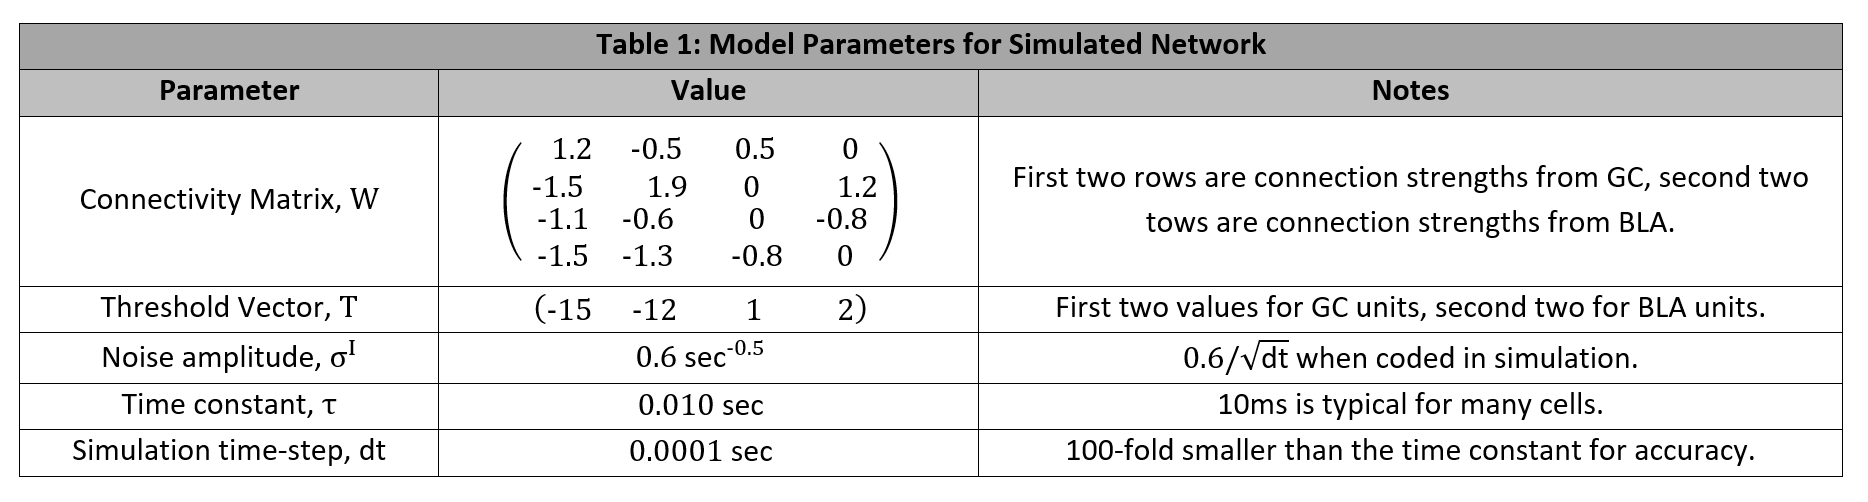
\includegraphics[width=\linewidth]{mahmood_22_figures/table1.PNG}
\end{tabular}
\noindent\underline{Phase Coherence for Network Model}
The simulation described above was used to generate 20 trials of neural activity. The activity of both units in each “region” was summed to produce a single time-series which was treated as an analog for LFP. This LFP was then bandpass filtered (10-40 Hz) and subjected to a Hilbert transform, and instantaneous phase was estimated using the analytical signal from the transform. Since latencies of state transitions in the simulated activity are random (unlike experimental data where they are roughly bounded in latency and occur in a sequential order, a fact likely related to the model’s omission of biological processes with longer time constants, like synaptic depression/facilitation or firing rate adaptation), we calculated phase coherence for the simulated data in each state using windows of activity centered around the transition from the more$\rightarrow$less coherent state. Data across trials were aligned to state transitions from the more$\rightarrow$less coherent states and snippets with radius = 350ms (minimum duration of states across all trials) of the LFP phase were taken around the transition time. Inter-trial phase coherence calculation was performed on these aligned snippets as described above.

\smallskip
\noindent\textbf{Data Availability}\par
\noindent We have structured our electrophysiology datasets in a hierarchical data format (HDF5) and are hosting the files on a university-wide network share managed by Library and Technology Services (LTS) at Brandeis University. These HDF5 files contain our electrophysiology recordings, sorted spikes, single-neuron and population-level analyses (and associated plots and results). These files are prohibitively large to be hosted on a general-purpose fileshare platform --- we request anyone interested in our datasets to contact the corresponding author, Donald Katz (dbkatz@brandeis.edu) who can put them in touch with LTS in order to create a guest account at Brandeis through which they can securely access our datasets (hosted on the katz-lab share at files.brandeis.edu). Code to perform the network model simulations can be found at \url{https://github.com/primon23/Two_State_Oscillators}.

\section{Results}
In order to appropriately contextualize our novel central hypothesis and analysis, we build the following accounting of the Results in a step-by-step manner. We start by replicating/confirming basic results from our prior work (Figs. 3.2 \& 3.3) and move on to testing basic questions concerning whether BLA responses show within-trial firing-rate transitions that could conceivably be coupled with those of GC (Figs. 3.4 \& 3.5). From there, we move on to using field-standard techniques to test whether GC and BLA responses show simple trial-to-trial coherence (Fig. 3.6), and whether coherence changes from one response epoch to the next (Figs. 3.7 \& 3.8). Once epoch-specificity of response coherence is established, we move on testing whether BLA-GC coupling during taste processing is specifically instantiated in the synchrony of transitions into and out of the GC palatability-related epoch, and whether the entirety of these phenomena is truly consistent with the function of tightly coupled networks (Figs. 3.9 \& 3.10).

\subsection{Simultaneous single-neuron ensemble recordings from BLA and GC}

\begin{figure}
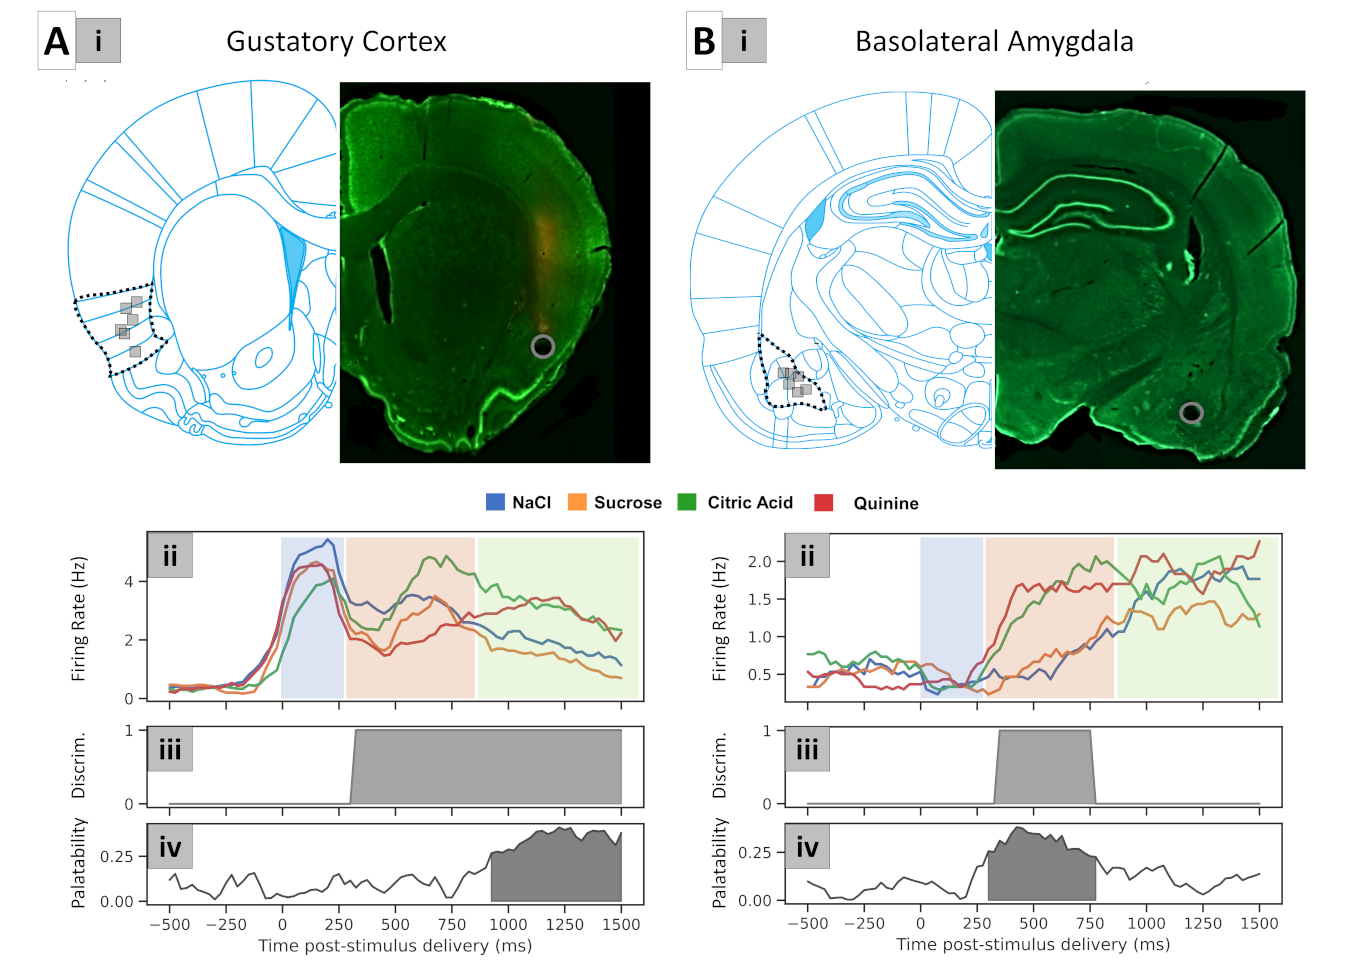
\includegraphics[width=\linewidth]{mahmood_22_figures/fig2-0.png}
\caption{\textbf{Histology and example PSTHs from recorded regions.} Column \textbf{A} is GC; column \textbf{B} is BLA. \textbf{(i)} Schematics and sample histology (x2 magnification) showing electrode bundle placements. Brain slices were registered to brain atlas schematics at 1.4 mm anterior to bregma for GC and 3.00 mm posterior to bregma for BLA. Dashed lines outline GC and BLA, with gray squares showing the final locations of each electrode bundle. Gray circles in the photomicrographs outline electrolytic lesions (schematics were modified from \cite{paxinos2007a}).  \textbf{(ii)}: PSTHs for representative GC and BLA single-neuron responses to each taste. Previously described response epochs (e.g., \cite{katz2001a}) are denoted with different colored shading behind the PSTHs. \textbf{(iii)}  Boolean timeseries reflecting whether neural activity significantly differentiates tastants (0 = no, 1 = yes) at a particular time point, with shading emphasizing periods of significant differences among responses. \textbf{(iv)} Correlation of neural activity with taste palatability (see Methods) through time; shaded regions denote periods of significant correlation.}
\label{fig:wrapfig}
\end{figure}

We isolated multiple single neurons simultaneously from both GC and BLA in 6 rats. Electrode bundle tip placements are shown in the top panels of Fig. 3.2: a coronal schematic of the regions (GC: Fig. 3.2A.i, BLA: Fig. 3.2B.i), with the locations of all bundle tips marked, is displayed in the left half of each panel; the right half of each panel is a photomicrograph showing an example placement. 

The rest of Fig. 3.2 presents representative recordings from each region. Fig. 3.2A.ii and B.ii show overlain peri-stimulus time histograms (PSTHs) of example GC and BLA neuron responses to each taste. The colors behind the PSTHs show the average periods of GC coding epochs described previously (\cite{katz2001a,fontanini2009a,sadacca2012a}). Note that both GC and BLA responses re-arrange themselves (i.e., the ordering of which tastes induce the larger/smaller response magnitudes changes, y-axis) around the times of epochal boundaries. The nature of the “coding” performed by each neuron changes with these epochal re-arrangements, as well (\cite{katz2001a,sadacca2012a,moran2014a,li2016a}); in GC, the early epoch has little taste specificity, but the middle epoch responses “code” at least a subset of tastes distinctly, and in the late epoch responses become generally organized by palatability (note, for instance, in Fig. 3.2A.ii that the late response is ordered from most aversive to most palatable --- the strongest response is to quinine, followed in order by citric acid, NaCl, and sucrose). In BLA, meanwhile, palatability-related responses appear in the middle epoch, and (unlike the GC responses) primarily reflect strong responses to tastes of only one (in this case, negative) valence; both of these aspects of BLA taste responses replicate previous investigations (\cite{fontanini2009a}).

These findings are statistically confirmed by analyses summarized in the panels below the PSTHs. The middle row (“Discrim” in the y-axis, Fig. 3.2A.iii and B.iii), which plots the significance (p\(<\)0.05) of a moving window of ANOVAs for Tastes, reveals that the responses displayed in Fig. 3.2A-B.ii become distinctly taste-specific starting at approximately 250 msec after taste delivery (i.e., at the start of the 2nd epoch; the BLA neuron stops doing so at the end of this epoch); the bottom panels (“Palatability”, Fig. 3.2A.iv and B.iv) which plot Pearson’s R between the known palatability of each taste and the neuron’s response to each taste --- i.e., the correlation (shaded region, p\(<\)0.05) between the two variables --- show that the palatability-relatedness of the GC responses becomes significant a little before 1000 msec after taste delivery (i.e., at the onset of the 3rd [late] epoch), and that the palatability-relatedness of the BLA responses is significant for the one-epoch  entirety (middle epoch) of the taste-specific response. Again, these results confirm findings published in multiple previous papers (\cite{katz2001a,grossman2008a,fontanini2009a,sadacca2012a}), and motivate our basic hypothesis that the systems-level mechanisms of taste coding will intrinsically involve epoch-specific processes.

A good deal of previous research has demonstrated that taste-response epochs translate into this sequence of states (each lasting hundreds of msec) in single-trial evoked GC ensemble activity (\cite{jones2007a,sadacca2016a,mukherjee2019a}), separated by sudden (50-200 msec) coherent firing-rate transitions (spontaneous GC activity also contains such transitions; see \cite{camera2019a,mazzucato2015a}). We note here that we use the term “epoch” to describe periods of distinct activity seen in single neuron PSTHs (Fig. 3.2), whereas “state” is a term borrowed from modelling literature and is used here to describe simultaneous changes in the recorded neural population activity while accounting for temporal variation at the single trial level. However, since state transitions correspond to epoch transitions across trials (on average, see Fig. 3.9C and D for a comparison of average state-transition times in our data and previously shown epochal-transition times), it is sometimes difficult to cleanly delineate single-trial from trial-averaged analyses; in these cases, we use the term that seems most appropriate.

These state transitions represent an integral part of neural activity, in that they both predict the onset of (\cite{sadacca2016a}) and drive (\cite{mukherjee2019a}) consumption-related behavior --- that is, rather than being trivial reflections of mouth movements, the dynamics represent the processing of tastes that leads to discriminative mouth movements (see also (\cite{jones2007a,katz2001a}). The seeming “ramping onset” of the above-described late epoch containing palatability-related firing (see Fig. 3.2) proves to be an artifact of averaging across the large trial-to-trial variability (on the order of hundreds of milliseconds) in the latency of this sudden transition (\cite{jones2007a,sadacca2016a}). Furthermore, because this phenomenon is not sparse --- approximately 50\% of the neurons in an ensemble will change their firing rates at any particular transition --- it can be reliably observed in sub-ensembles as small as 6 simultaneously-recorded neurons (\cite{jones2007a}). 

\begin{figure}
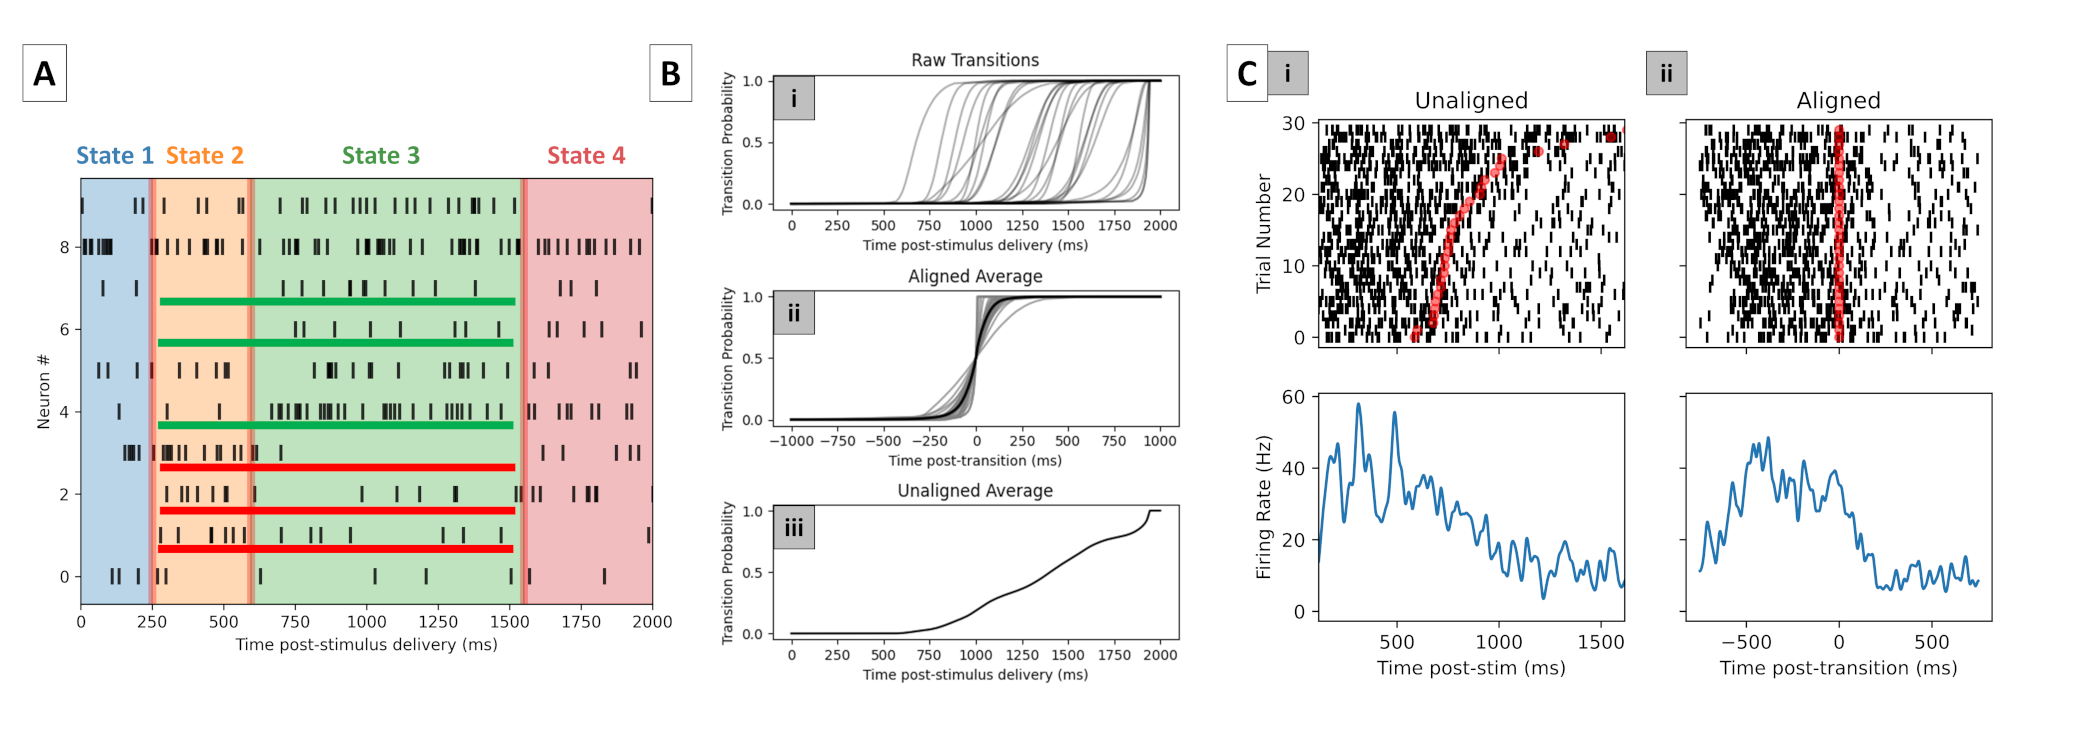
\includegraphics[width=\linewidth]{mahmood_22_figures/fig3-0.png}
\caption{\textbf{GC evoked population activity contains sudden state transitions.} \textbf{(A)} A single trial of GC taste-evoked activity in 10 simultaneously recorded single neurons. Inferred states (here identified using an ensemble change-point algorithm) are indicated in overlain shading. For the transition leading into the period of palatability-related activity (i.e., from State 2$\rightarrow$3), spike trains that increased in firing rate are underlined in green, and spike trains that decreased in firing rate are underlined in red. \textbf{(B) (i)}  Identified time-courses for the State 2$\rightarrow$3 transition in 30 trials for a single ensemble. \textbf{(ii)} aligning the middle (i.e., 0.5 probability) of the transitions shows that they typically occur suddenly. \textbf{(iii)} when averaged across data synchronized to stimulus onset, however, the transition appears smooth and slow (similar to neural activity in trial-averaged PSTHs). \textbf{(C) (i)} The raster plot (above) and PSTH (below) for a single, representative GC neuron that shows a sudden decrease in its firing rate occurring at variable latencies across trial. The time of the transition, inferred by the change-point algorithm on activity of the entire simultaneously recorded ensemble, is shown with a red hash mark. \textbf{(ii)} By aligning activity to calculated transition times (producing a “peri-transition time histogram”), the sharp decrease in neural activity across the transition can be better appreciated.}
\label{fig:wrapfig}
\end{figure}

Once again, the current data replicate these findings (Fig. 3.3), showing that even a small ensemble of simultaneously-recorded GC neurons (here, 10-again, almost 2x the number of neurons needed to resolve this phenomenon; (\cite{jones2007a})) can be observed to undergo sudden, coherent firing-rate changes in the process of responding to tastes (Fig. 3.3A). The states and state transitions identified by our change-point algorithm are overlain on the ensemble raster plot, and the 6 (of 10; 60\%) neurons that significantly increased or decreased their firing rates at the time of the transition into the 3rd (putative palatability-related) state are indicated with green or red lines, respectively (note the sudden increase in the rate of spiking in neurons 4, 6, and 7, and the simultaneous decrease in firing rate in neurons 1, 2, and 3) under their spike trains. The algorithm was able to progress to near-perfect confidence in the transition across an extremely short time interval in almost every trial (Fig. 3.3B.i), which is to say that these changes in neural activity are, on average, very sudden on a single-trial basis (Fig. 3.3B.ii); because the latency of the transition could vary wildly from trial-to-trial (Fig. 3.3B.i), however, the onset of the post-transition state appears to be a slow-ramping onset of the late epoch when averaged across trials synchronized to stimulus delivery (Fig. 3.3B.iii). 

Once calculated from the ensemble data, the time of transitions could then be used to directly illustrate the sharpness of the firing-rate changes in even single-neuron data. Fig. 3.3C shows a representative GC neuron: note that the firing-rate change that seems like a slow ramp in data synchronized to stimulus delivery (Fig. 3.3C.i: “Unaligned” rasters above and associated peri-stimulus time histogram below) is in fact precipitous when the trial-to-trial variability of that change’s latency is accounted for (Fig. 3.3C.ii: “Aligned” rasters and associated peri-transition time histogram). Keep in mind that this change is not caused by the stimulus being removed from the tongue: it occurs at least a full second before swallowing, and both precedes and reliably predicts (\cite{sadacca2016a}), as well as participates in driving (\cite{mukherjee2019a}) discriminative oral behaviors.

\subsection{BLA activity contains trial-specific, sudden ensemble firing-rate transitions}
Having re-confirmed that GC epochal dynamics reflect sequences of single-trial states, and en route to assessing the coordination between BLA and GC neural responses and testing our hypothesis that BLA state transitions are coupled to those in GC, it is necessary that we determine whether the sort of nonlinearities in firing rate which have been extensively described in GC (Fig. 3.3; see also \cite{jones2007a,sadacca2016a}) also truly characterize BLA taste responses. That is, we must first test whether evoked BLA activity, which involves epochal dynamics that are similarly timed to those in GC (see Fig. 3.2 for single-neuron examples of the similarity between BLA and GC dynamics; see also \cite{fontanini2009a}), are well described as sudden ensemble state transitions in single trials. Only if the population dynamics of BLA taste-evoked responses also consist of sudden transitions between a small number of ensemble states (a hypothesis that has not yet been tested) is our most novel hypothesis tenable.

To this end, we evaluated the spiking activity of BLA ensembles using the same changepoint model designed to detect coherent ensemble transitions in GC data. To ensure robust sampling of BLA population activity, this set of analyses was performed on data from a separate group of animals with bilateral BLA electrode implants (2 animals, 9 recording sessions; however, all results reported in this analysis were qualitatively similar to those obtained using unilateral BLA populations taken from BLA-GC dual region recordings --- see below). First, we fit a battery of models containing 2-10 states to the evoked responses from the BLA ensembles, and compared the goodness-of-fit of the probabilistic models (quantified using the ELBO; see Methods) to that of identical analyses performed on control datasets made by shuffling either whole trials or single spikes between trials for the same neuron (both manipulations preserve the across-trial dynamics and have equivalent PSTHs to the actual data; Fig. 3.4A). Performing this set of analyses allowed us to test whether the real data were better fit by the sudden transition model than one would expect by chance. We predicted that the unmanipulated data would achieve a higher goodness-of-fit to the sudden state change model.

\begin{figure}
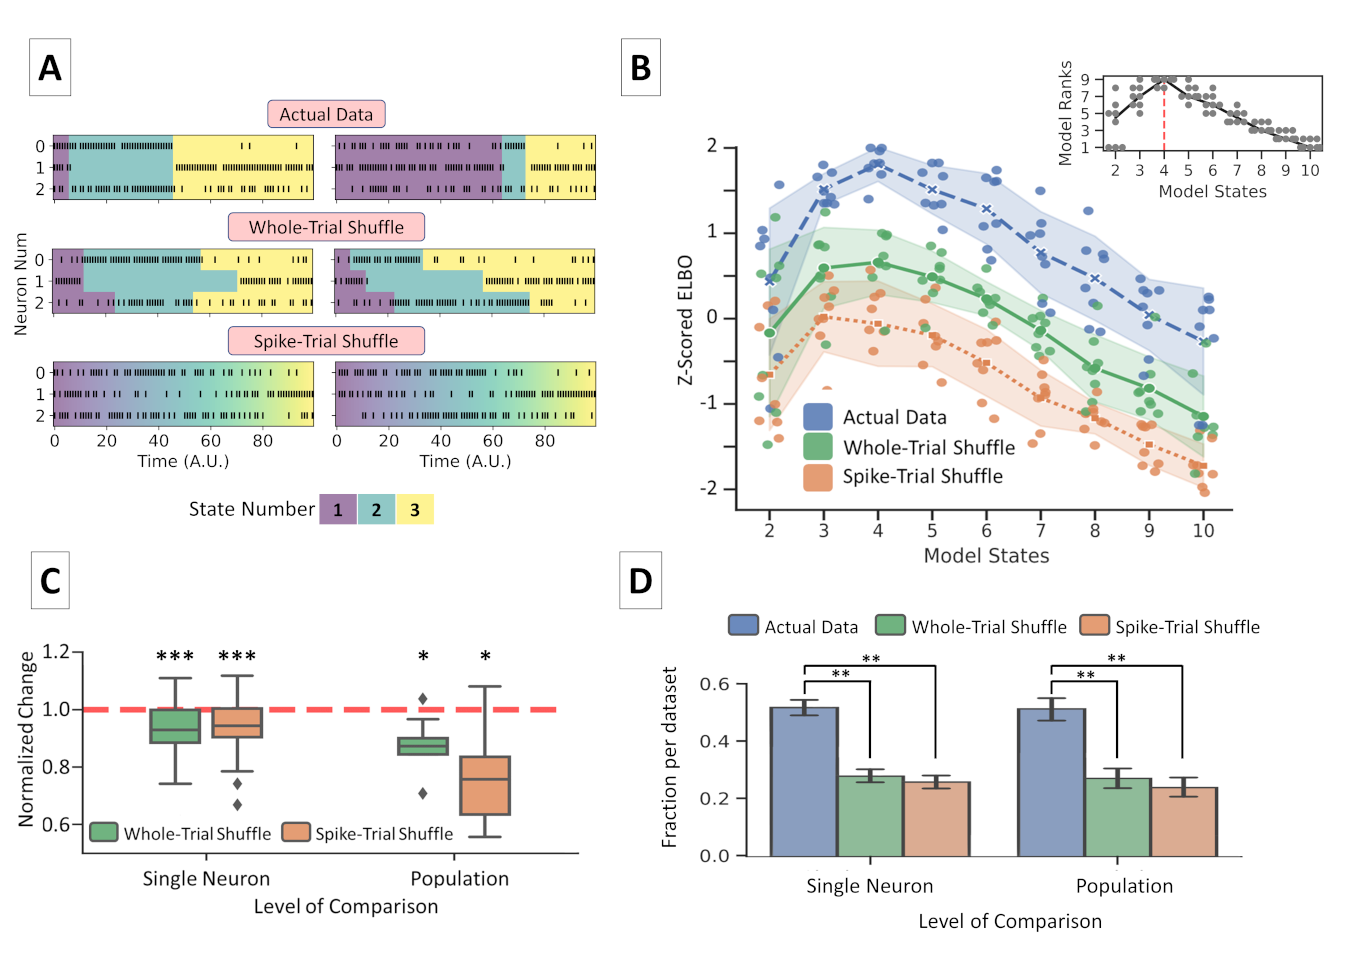
\includegraphics[width=\linewidth]{mahmood_22_figures/fig4-0.png}
\caption{\textbf{BLA population responses can validly be characterized as progressing through a sequence of state transitions.} \textbf{(A)} Visualization of how the actual data were transformed by the different shuffling procedures. Raster plots are overlayed with colors identifying states for the neural population; two trials (one in each column) are shown. \underline{Actual Data:} State-transitions are hypothesized to occur coherently across all neurons for the same trial. \underline{Whole-Trial Shuffle:} State-transitions are mismatched between neurons on the same trial. \underline{Spike-Trial Shuffle:} Sharp, trial-variable state-transitions have been destroyed by changing in which trial each particular spike occurred, largely leaving smooth changes in the neural activity which are consistent across trials. A.U. : Arbitrary Units  \textbf{(B)} ELBO values for 2-10 state models fit to the actual data and surrogate datasets. Note that the ELBO (unlike model likelihoods) penalizes more complicated models, allowing us to visualize peak fit rather than seeking an actual elbow in monotonically increasing functions. Inset) Ranks for models with 2-10 states. Models with 4 states consistently show the highest ranks across the dataset. Solid black line shows median rank per state. \textbf{(C)} Comparison of average, normalized changes in single-neuron and population vector firing rates in the vicinity (from 500ms before to 500 msec after) of transitions. Firing-rate changes across transitions are consistently diminished by shuffling, a decrement that is particularly noticeable at the population level. Edges of boxes show 1st and 3rd quartiles, and the horizontal line through the boxes shows the median. The dashed red line denotes the (normalized) firing-rate changes in the actual data. * = p\(<\)0.05, *** = p\(<\)0.001, for mean value is different from 1.0 \textbf{(D)} Comparison between actual data and shuffled surrogate datasets for which dataset contained the higher number of "larger“ transitions. Unperturbed BLA datasets consistently had more transitions with largest changes in firing rate (Mean ± SEM, **: p\(<\)0.01).}
\label{fig:wrapfig}
\end{figure}

This analysis revealed that models with 4 states had the highest ELBO-that 4-state models best describe BLA population activity for the 2000ms of post-stimulus activity we have used in this study (Fig. 3.4B, see Table 2 for statistics used to test these effects). Note that only 3 of these states typically appeared in the first 1500 msec-that is, in the period leading up to and including the GC “palatability-related” state-and that while we are interested in the transition out of that “palatability-related” state, we are not yet prepared to interpret the state following (which is post-decision). This number of states accords well with results from HMM modeling of GC activity (\cite{jones2007a,sadacca2016a}), supporting our suggestion that GC and BLA taste-response dynamics are similar in kind (and demonstrating that these results hold across very different analysis techniques). Furthermore, this fit was significantly higher (as was the relative advantage of the 4-state model) than that achieved by even the trial-shuffled surrogate dataset (F(2,20)=26.9, p=2.13x10$^{-6}$, 2-way repeated measures ANOVA for Shuffle Type and Number of States, n=9 recordings across 2 animals), which left each trial’s spike trains intact (Fig. 3.2), eliminating only the between-neuron coherence of single-trial dynamics. 

\begin{tabular}
\centering
    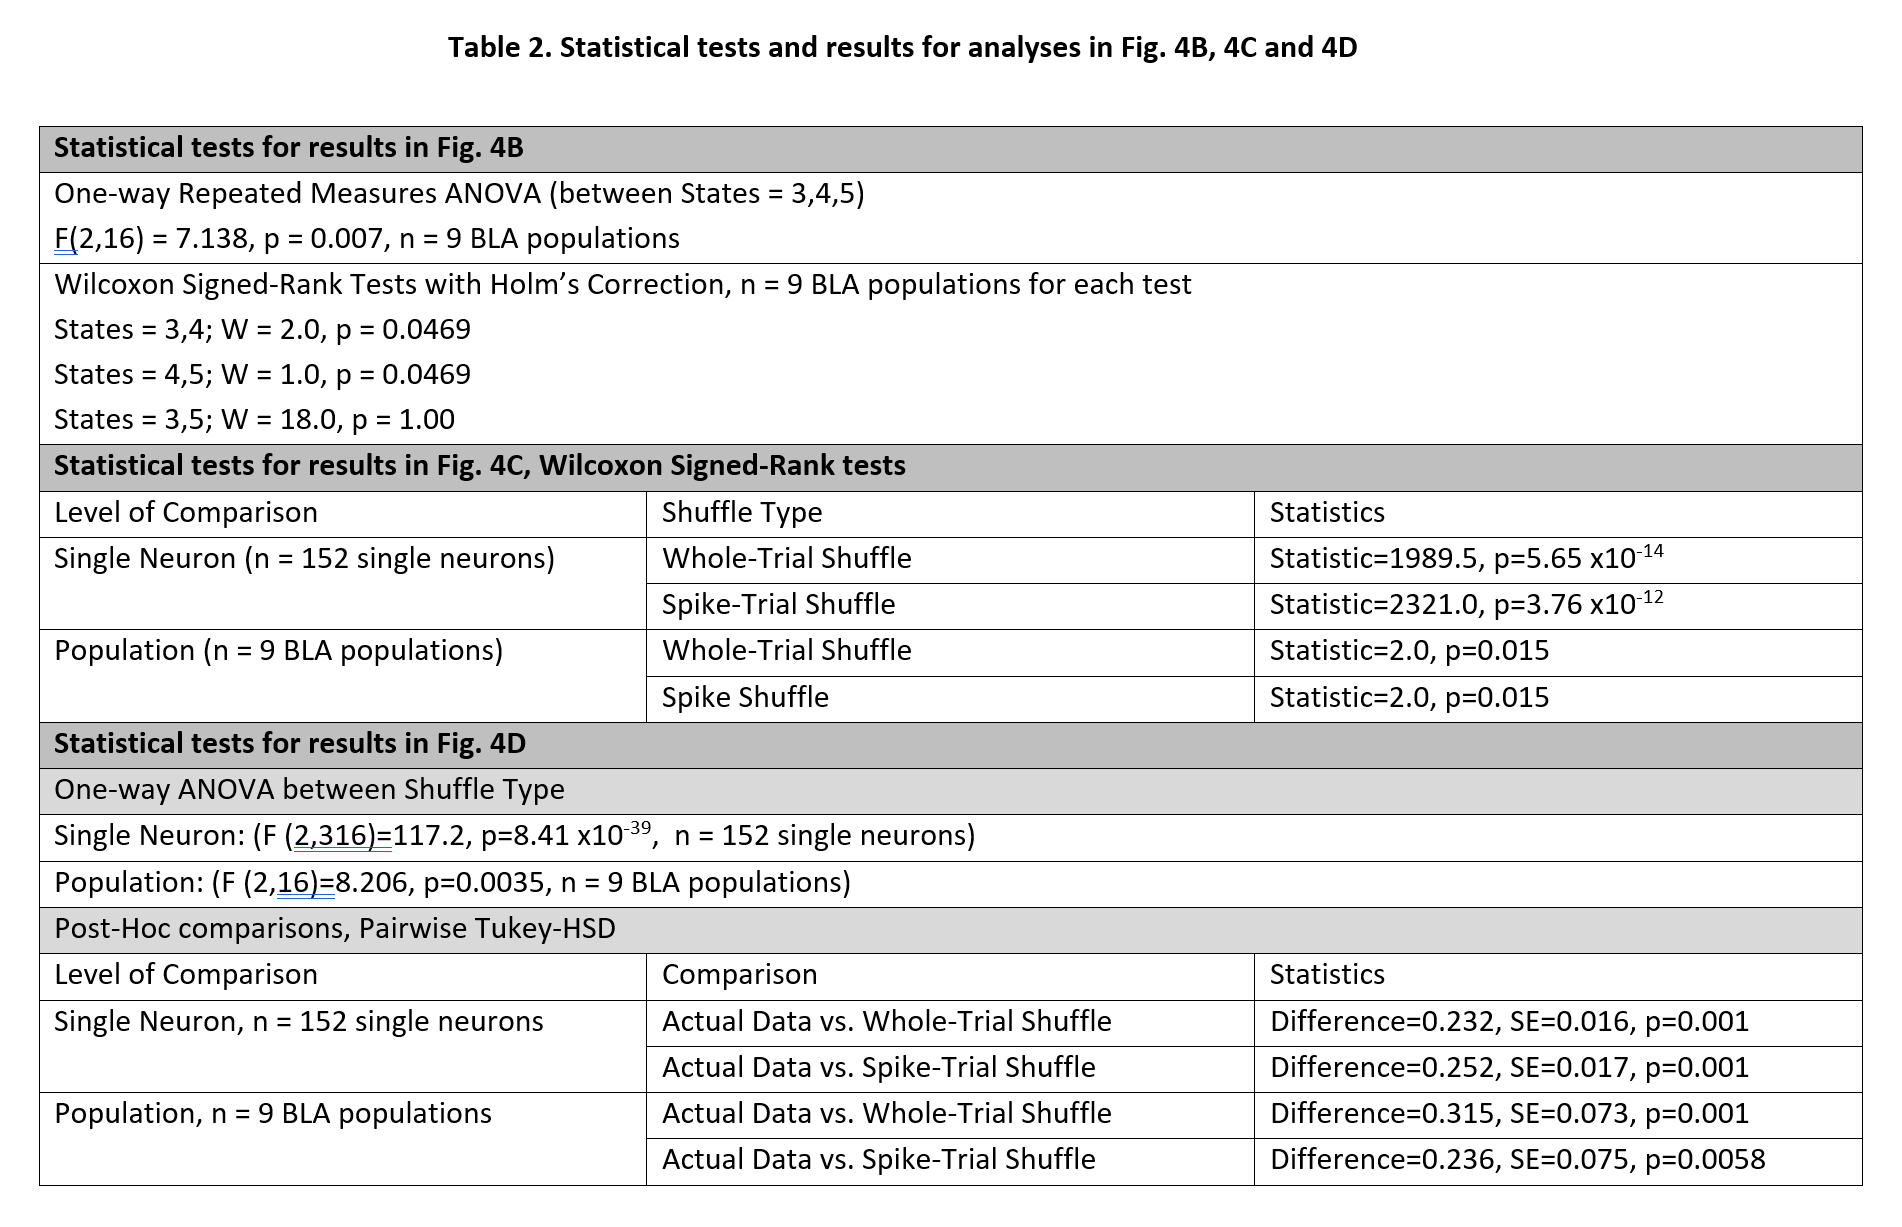
\includegraphics[width=\linewidth]{mahmood_22_figures/table2.PNG}
\end{tabular}

We further evaluated the BLA ensemble data by comparing the magnitude of firing rate changes across state transitions identified by this optimal 4-state changepoint model (see \cite{sadacca2016a} for similar analysis of GC responses), compared to those observed in surrogate datasets. We predicted that both the average magnitude of transition-aligned changes in firing rates and the quantity of transitions showing larger changes in firing would be higher for the “actual” data than for the surrogate datasets in which we disrupted the coherence of single-trial changes in population activity. Our results confirmed these predictions: compared to the surrogate datasets, neurons and ensembles in the actual, unmanipulated BLA data showed consistently larger changes in firing rate across transitions (Fig. 3.4C; see Table 2 for an accounting of the extensive statistical analyses used in these tests); furthermore, the percentage of BLA single neurons and ensembles for which changes in firing rate across transitions were largest in the actual data was more than twice that for either shuffled dataset (Fig. 3.4D; again, see Table 2). 

These findings suggest that BLA ensemble taste responses are well described as consisting of sudden, coherent firing-rate transitions in single trials. Fig. 3.5A shows a representative ensemble taste response from 8 simultaneously recorded BLA neurons that clearly involves rapid state transitions, one of which occurs at around the average time of GC transitions into palatability coding (see Fig. 3.2); at this transition, 5 out of 8 neurons underwent either an increase or decrease of firing rate simultaneously (for another, neuron #3, the increase was almost but not quite significant). As in GC (Fig. 3.3; see also \cite{jones2007a,sadacca2016a}), these transitions were variable in latency across trials (Fig. 3.5B.i), such that while the average transition time was brief (Fig. 3.5B.ii), averaging across trials synchronized to stimulus delivery made that transition time appear artifactually slow (Fig. 3.5B.iii).

\begin{figure}
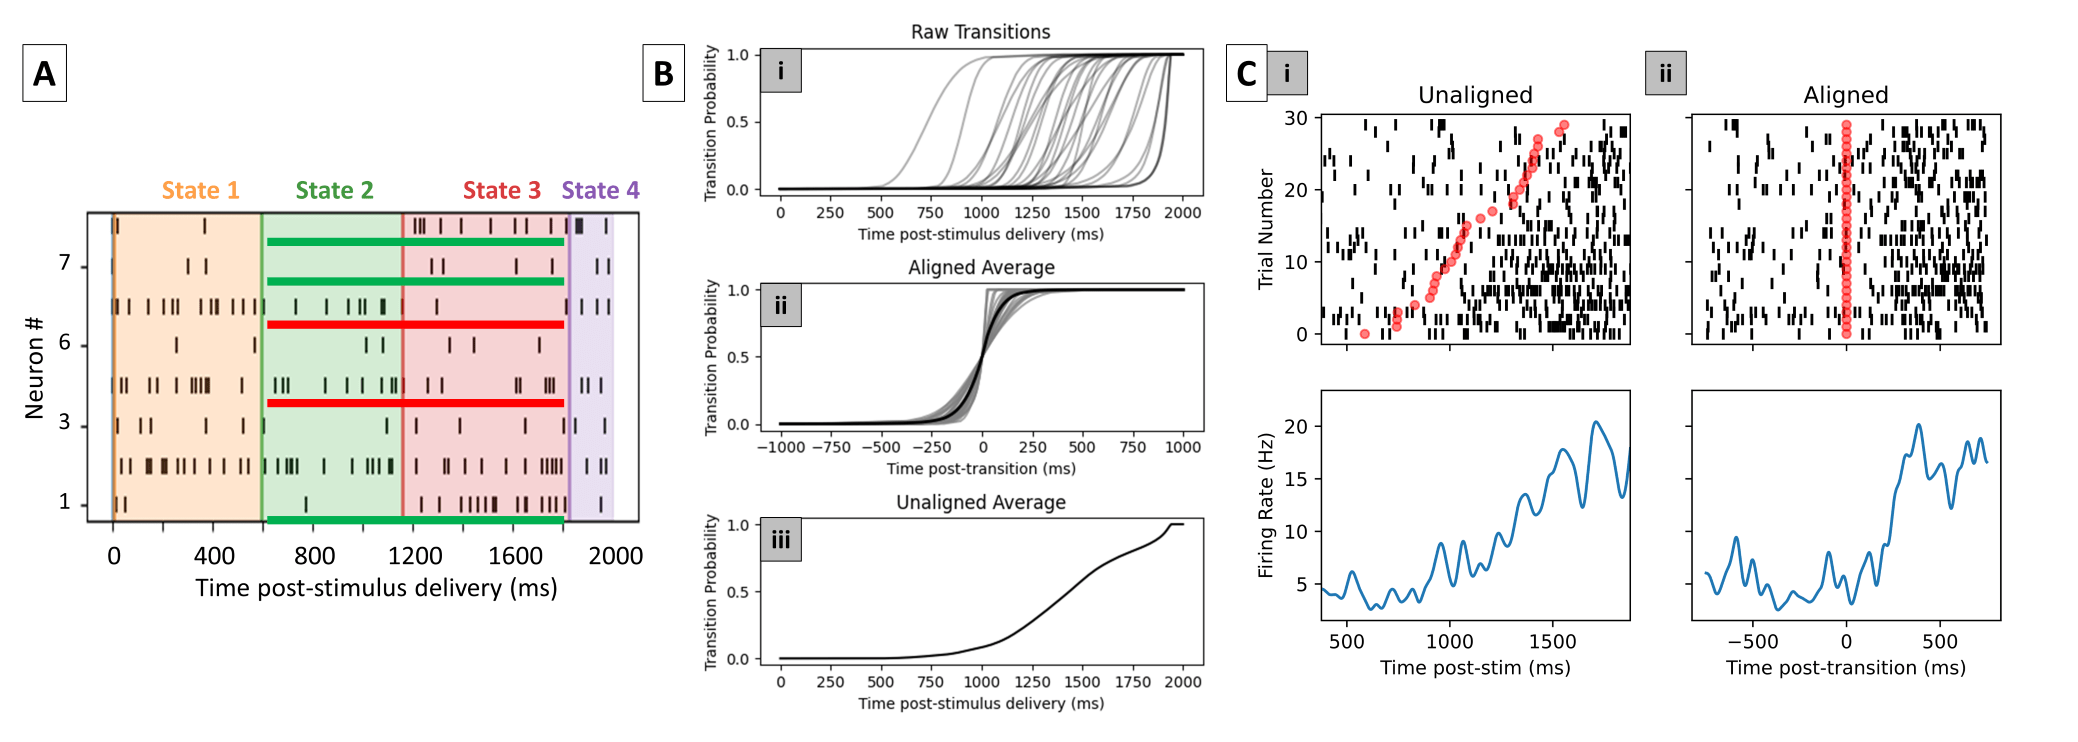
\includegraphics[width=\linewidth]{mahmood_22_figures/fig5_corrected_rescaled.png}
\caption{\textbf{BLA evoked population activity contains sudden state transitions. (A)} A single trial of BLA taste-evoked activity in 8 simultaneously recorded single neurons. Inferred states (here identified using an ensemble change-point algorithm) are indicated in overlain shading. For the transition leading into the period of palatability-related activity (i.e., from State 2$\rightarrow$3), spike trains that increased in firing rate are underlined in green, and spike trains that decreased in firing rate are underlined in red. \textbf{(B) (i)} Identified time-courses for the State 2$\rightarrow$3 transition in 30 trials for a single ensemble. \textbf{(ii)} aligning the middle (i.e. 0.5 probability) of the transitions shows that they typically occur suddenly. \textbf{(iii)} when averaged across data synchronized to stimulus onset, however, the transition appears smooth and slow (similar to neural activity in trial-averaged PSTHs). \textbf{(C) (i)} The raster plot (above) and PSTH (below) for a single, representative BLA neuron that shows a sudden increase in its firing rate occurring at variable latencies across trial. The time of the transition, inferred by the change-point algorithm on activity of the entire simultaneously recorded ensemble, is shown with a red hash mark. \textbf{(ii)} By aligning activity to calculated transition times (producing a “peri-transition time histogram”), the sharp increase in neural activity across the transition can be better appreciated.}
\label{fig:wrapfig}
\end{figure}

Finally, we again fed back the results of this ensemble analysis to directly illustrate the sharpness of single-neuron firing changes across transitions. Fig. 3.5C shows, for one representative BLA neuron, that firing-rate changes that seem like slow ramps in data synchronized to stimulus delivery (Fig. 3.5C.i; “Unaligned” rasters and associated peri-stimulus time histogram) are in fact precipitous when the trial-to-trial variability of that change’s latency is accounted for (Fig. 3.5C.ii; “Aligned” rasters and associated peri-transition time histogram). While we have no current explanation for the apparent slight delay in this particular BLA neuron’s firing-rate change (we suspect that the answer lies in compromises made by the algorithm in settling on a “best guess” of transition time), it is clear that BLA ensembles, like GC ensembles, respond to tastes with sequences of states separated by sudden state transitions.

\subsection{BLA and GC responses show strong trial-to-trial coherence}
The above data motivate our hypothesis that taste processing involves BLA-GC coupling of the brief transitions into the state that, in GC, predicts and controls consumption behavior. But given that the vast majority of published studies assessing multi-region coordination have done so not in terms of momentary coupling-they have instead focused on multi-second responses, with quantification performed via evaluation of the magnitude of correlation between spike counts in simultaneously-recorded pairs of neurons (\cite{averbeck2006a,averbeck2006b}), or alternatively via evaluation of similarity in local field potentials (LFP) simultaneously recorded from the regions under investigation (\cite{place2016a}) --- we first assessed whether GC taste processing is coherent with that of BLA according to these standard metrics. To maximize our ability to compare our results to those of these earlier studies, we began our investigation of BLA-GC taste-response coupling by looking at these broader measures, and then moved on (in the following sections) to testing the epochal specificity of this coherence, a result that would more directly motivate our ultimate test of the hypothesized synchronous transitions BLA-GC transitions into the behaviorally-relevant state.

We first considered the trial-wise strength of coordination between BLA and GC, by investigating trial-to-trial spike-count correlations (using the 0-2000 ms post-stimulus time-period, which is the period of the most prominent taste-evoked response) for every simultaneously-recorded BLA-GC pair of neurons, thereby testing the broad hypothesis that BLA and GC responses rise and fall in a correlated (or anti-correlated) manner from trial-to-trial. The two example BLA-GC neuron pairs shown in Fig. 3.6A in fact demonstrate strong coherence on this time scale: the trial-to-trial firing rates of the pair on the left are (significantly) anti-correlated, a fact that can be particularly well appreciated in the scatterplot of BLA and GC firing rates (each dot reflects one trial) below the trial-to-trial chart of responses; the pair to the right is similarly (albeit in this case positively) correlated. 

\begin{figure}
\centering
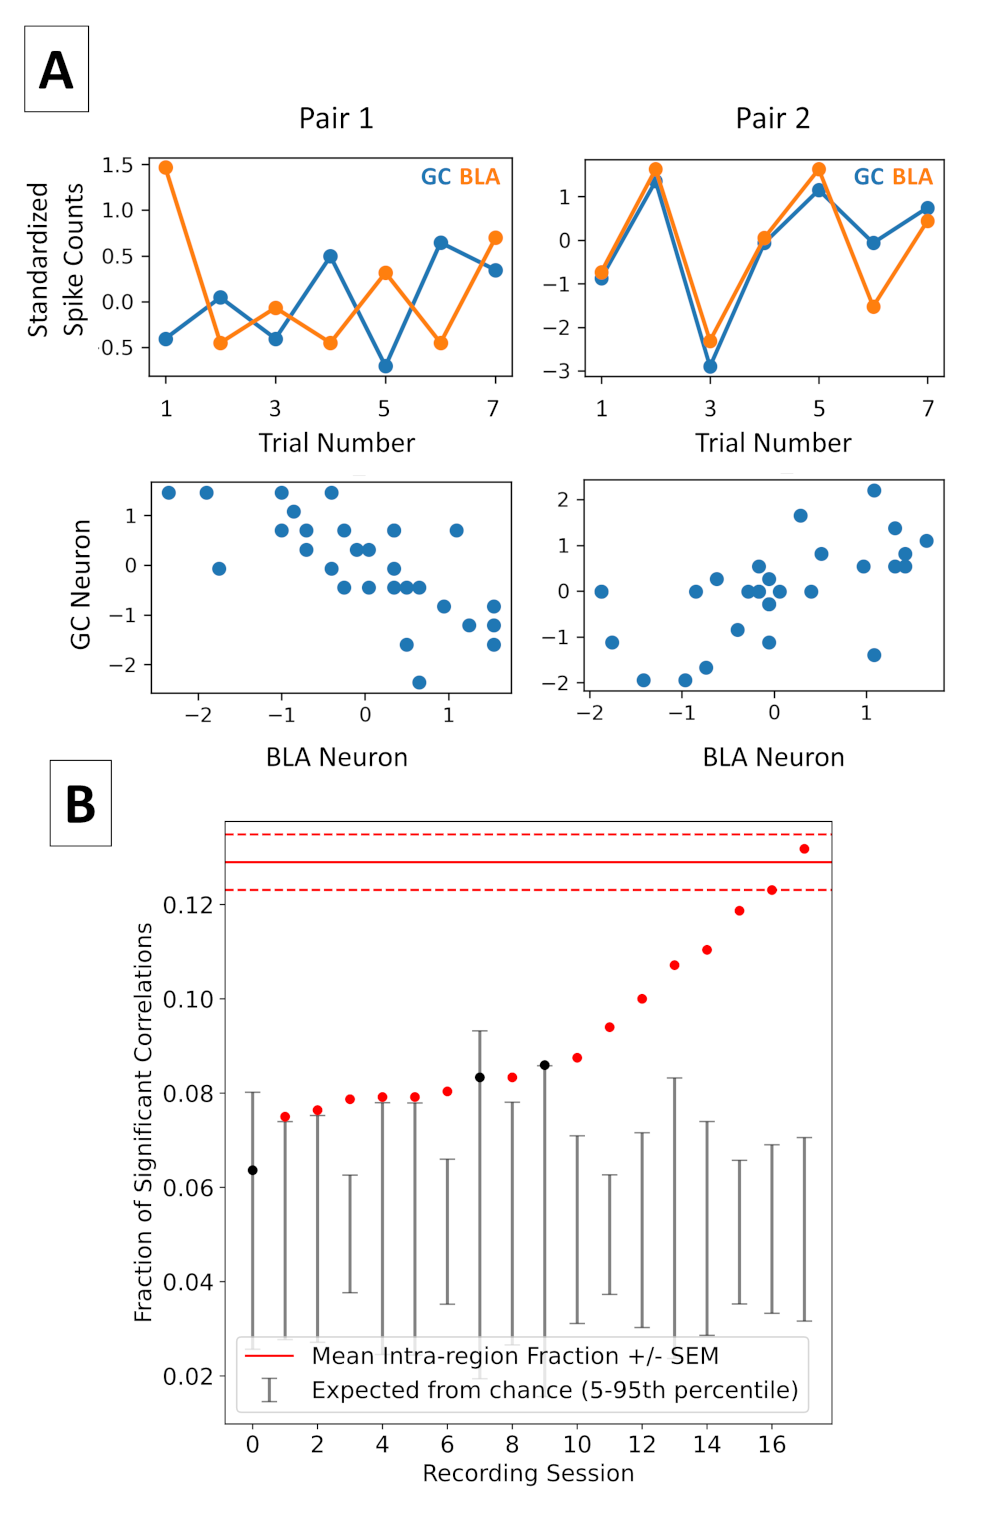
\includegraphics[width=0.5\linewidth]{mahmood_22_figures/fig6-0.png}
\caption{\textbf{BLA and GC show strong spike-count correlations on a trial-matched basis. (A)} Top row: Representative timeseries of (standardized) spike counts for two BLA-GC neuron pairs. Shown for each are consecutive sets of 7 trials (out of 30) showing negatively correlated (left) and positively correlated activity (right). Bottom row: Same data as top (but including all 30 trials) row plotted as a scatterplot showing all of the trials/pair; the negative (left) and positive (right) correlations in the scatterplot are easily seen. \textbf{(B)} A comparison of the fraction of significant correlations across all comparisons (neuron pairs x tastes) for trial-matched and trial-shuffled (i.e., GC trial 1 compared to BLA trial 4, etc) data. Trial-matched spike-count correlations (filled circles) are in all but 3/18 sessions significantly higher compared to the trial-shuffled comparisons (vertical lines); error bars show the 5-95th percentile interval of fraction of significant correlations per session expected by chance, red circles (n=15) show sessions for which the fraction was higher than expected by chance, and black circles (n=3) show sessions for which the value was within the chance interval. The interval marked by the horizontal dotted lines shows the Mean +/- SEM fraction of significant intra-region correlations (i.e., all BLA-BLA and GC-GC neuron pairs), included for reference.}
\label{fig:wrapfig}
\end{figure}

Across the entire sample, BLA-GC neuron pairs (averaged across all pairs in a single session) almost always showed higher spike-count correlations than did trial-shuffled data (Fig. 3.6B, 15/18 comparisons had values significantly higher than those expected by chance, n = 18 sessions from 6 animals), confirming that the taste responses of simultaneously-recorded BLA and GC single neurons are coupled in magnitude. Of course, either positive or negative correlations indicate connectivity at the single-neuron level, since a neuron pair can have either an effective excitatory or inhibitory connection between them; both connection types characterize projections connecting BLA and GC, and either can create coordinated dynamics between both regions (\cite{haley2016a,fu2020a}).

\subsection{The time-courses of BLA and GC taste responses are coupled}
The above analysis reveals a broad coordination in BLA-GC neural activity --- trial-to-trial differences in firing rates in BLA neurons, measured in stimulus-evoked responses separated by \(>\)20 seconds, predict trial-to-trial differences in firing rates in simultaneously recorded GC neurons. But this result falls short of revealing whether this amygdala-cortical coupling has anything specific to do with taste processing. It is possible that taste responses are simply “riding on” generally coupled excitability existing at long time-scales, not unlike that detected in studies of “resting-state network” dynamics (\cite{raichle2015a,seitzman2019a}). Given our proposal that a central feature of BLA-GC coherence is the specific coupling of state-to-state transitions, it is important to first test whether this inter-regional coherence is epoch-specific.

\begin{figure}
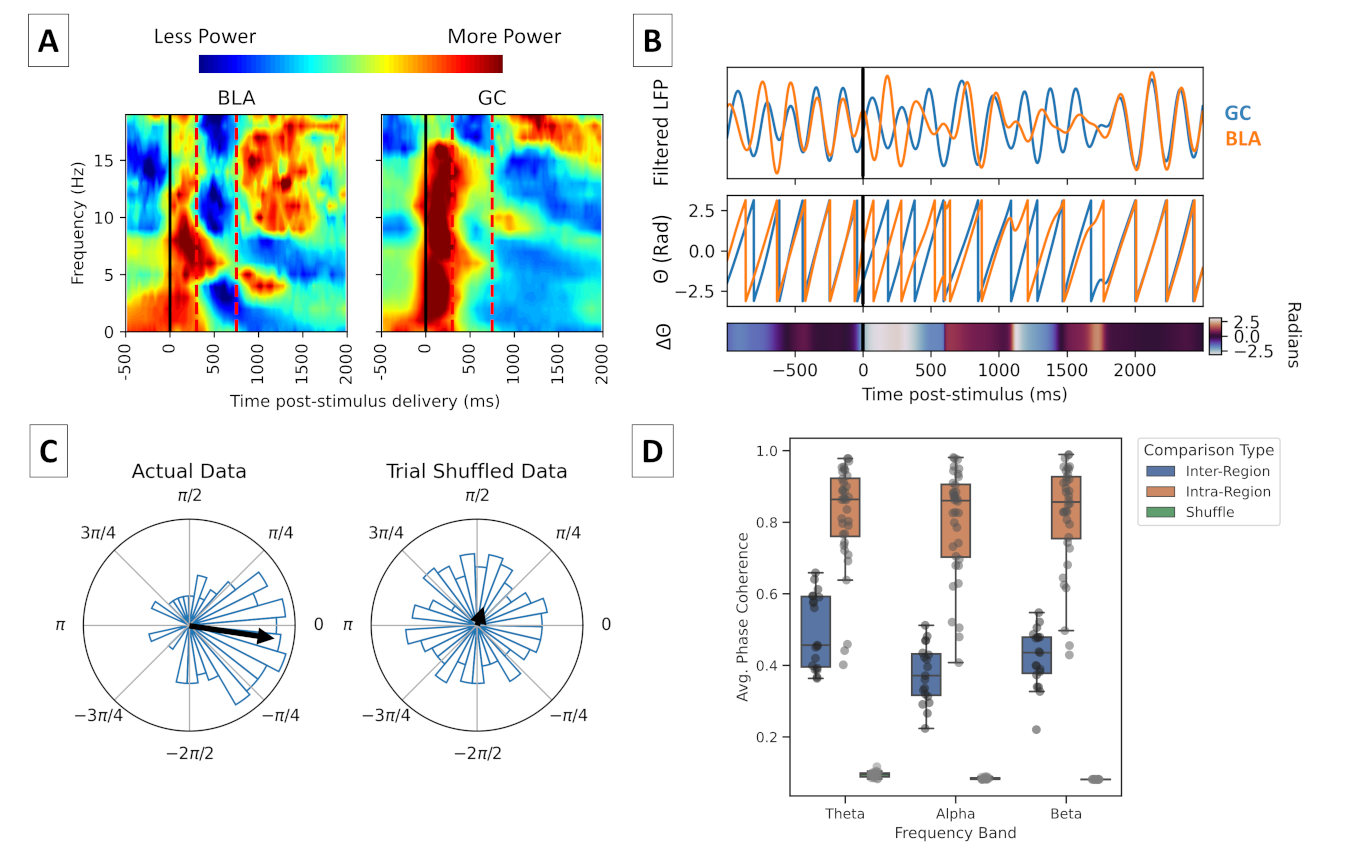
\includegraphics[width=\linewidth]{mahmood_22_figures/fig7-0.png}
\caption{\textbf{BLA and GC evoked LFP responses are similar on a trial-matched, but not trial-shuffled basis. (A)} Trial-averaged spectra of GC and BLA taste responses. Solid black lines mark taste delivery, and dashed red lines mark the average times of epoch onsets, which are well aligned with changes in the spectra in both regions. Power in each plot is Z-Scored by frequency for the time periods shown. \textbf{(B)} Calculation of BLA-GC phase difference for a single trial. Top panel shows filtered LFP (4-7 Hz) for each region, middle panel shows extracted phase (\Theta$), bottom panel shows phase difference (\Delta\Theta$) \textbf{(C)} Phase difference histograms (length of blue bars = frequency of occurrence) used to quantify similarity between GC and BLA LFP using average inter-trial phase coherence. Small phase differences (indicated by strong peaks in the polar histogram close to 0) indicate strong coherence. This is quantified using the magnitude of mean phase difference vector (black arrows). Data show the  distribution of phase differences for t=0ms post-stimulus delivery for actual and trial shuffled data. \textbf{(D)} Mean phase coherence for 0-2000ms post-stimulus delivery across frequency bands. The value of the trial-matched comparison is significantly higher than the trial-shuffled comparison, suggesting that there are similarities in the activity of both regions which are not present in “trial-averaged” data.}
\label{fig:wrapfig}
\end{figure}

We therefore moved next to examining coherence in the time-courses of taste-evoked responses, using analyses of local field potentials (LFPs) that have often been employed for such purposes (\cite{antzoulatos2016a,place2016a,saravani2019a}). Even casual scrutiny reveals what appear to be striking similarities in the (trial-averaged) spectral power/amplitude of BLA and GC field potentials (Fig. 3.7A). While the dominant frequencies differ between regions, in both regions the frequency spectra change repeatedly across the 1-1.5sec following stimulus delivery, in a manner that is well aligned with the approximate average timing of epochal transitions of ensemble firing described previously (see Fig. 3.2, and \cite{fontanini2009a,katz2001a,sadacca2016a}). 
These observations were statistically evaluated using quantification of the inter-trial phase coherence (\cite{stitt2017a,engel2020a,kramer2020a,zareian2020a}) between BLA and GC taste responses. Briefly, phase information for BLA and GC LFPs (across the 4-30 Hz band) was extracted using the Short Time Fourier Transform, after which phase differences between the two regions were calculated (Fig. 3.7B). These measurements were aggregated across all trials for each time-bin separately, and the variance was evaluated across post-stimulus time bins (see Fig. 3.7C); the tighter the resulting phase-difference distribution, the stronger the coupling. The results of this analysis revealed that, while inter-areal coherence (blue bars) was inevitably smaller than intra-areal coherence (tan bars), it was significantly larger than the (control) coherence between mismatched trials (Fig. 3.7D; it’s worth noting that this measurement likely under-estimates the true cross-coherence, because any epoch-to-epoch differences will add to the variance and reduce the across-trial average). This result held for all of the frequency bands that we assessed (theta: 4-7Hz, mu: 8-12Hz, beta: 13-25Hz, F(2,34)=654.5, p=7.21x10$^{-28}$ for “Comparison Type” using Repeated Measures ANOVA; for all pairwise comparisons p=1.61x10$^{-7}$ [all p-values are at the lower bound for numerical error], pairwise Mann-Whitney U Tests, n = 18 recordings across 6 animals). Qualitatively similar results were observed for simple cross-correlations between LFP power spectra for BLA and GC (data not shown). The trial-averaged time-courses of GC and BLA activity, as measured in evoked LFP activity, are coupled above and beyond overall magnitudes, in a manner that looks, at first blush, to be related to epochal processing (\cite{katz2001a,fontanini2009a,sadacca2012a}).  

\subsection{BLA and GC cross-coherence is epoch-specific}
Given the above, the fact that the different GC epochs have been shown to reflect distinct coding processes, and the likelihood that BLA is more integrally involved in the coding of palatability than taste identity (\cite{piette2012a,lin2021a}) , we hypothesized that, beyond the overall time courses being coupled, the cross-coherence between GC and BLA (evaluated in LFP time-courses) would itself be epoch-specific. 

Our test of this hypothesis is summarized in Fig. 3.8, which reveals that phase coherence between BLA and GC is in fact modulated in an epoch- (and, as it turns out, frequency-) specific manner by stimulus delivery. Changes in the theta (4-7Hz) band were centered largely on the initial (i.e., taste-nonspecific) epoch of the responses: in most (11/18) sessions, theta activity changed significantly from baseline; overwhelmingly (in 9/11 cases), these early-response changes involved a decrease in phase coherence. In the mu (7-11Hz) band, meanwhile, changes were centered on the later (palatability-specific, see \cite{katz2001a,sadacca2012a}) response epoch; these changes, which were even more ubiquitous than theta changes, in every case involved a decrease in coherence (see the right-hand panels of Fig. 3.8A-B, n = 18 recordings across 6 animals). A reduction in coherence following stimulus delivery was predictable given previous results showing that strong levels of inter-region coherence tend to be associated with states of “low cognitive engagement” such as sedation, epilepsy, and cognitive impairment (\cite{supp2011a,martinet2017a,arbab2018a}), as well as the fact that BLA and GC “encode” tastes non-identically – hence, their specific neural responses are likely to differ (see also Discussion). Note, however, that phase coherence always stays higher than random levels (BLA and GC are never functionally “disconnected”), and that state-specific reductions in coherence can be recapitulated in simple, tightly interconnected model networks (see below). 

\begin{figure}
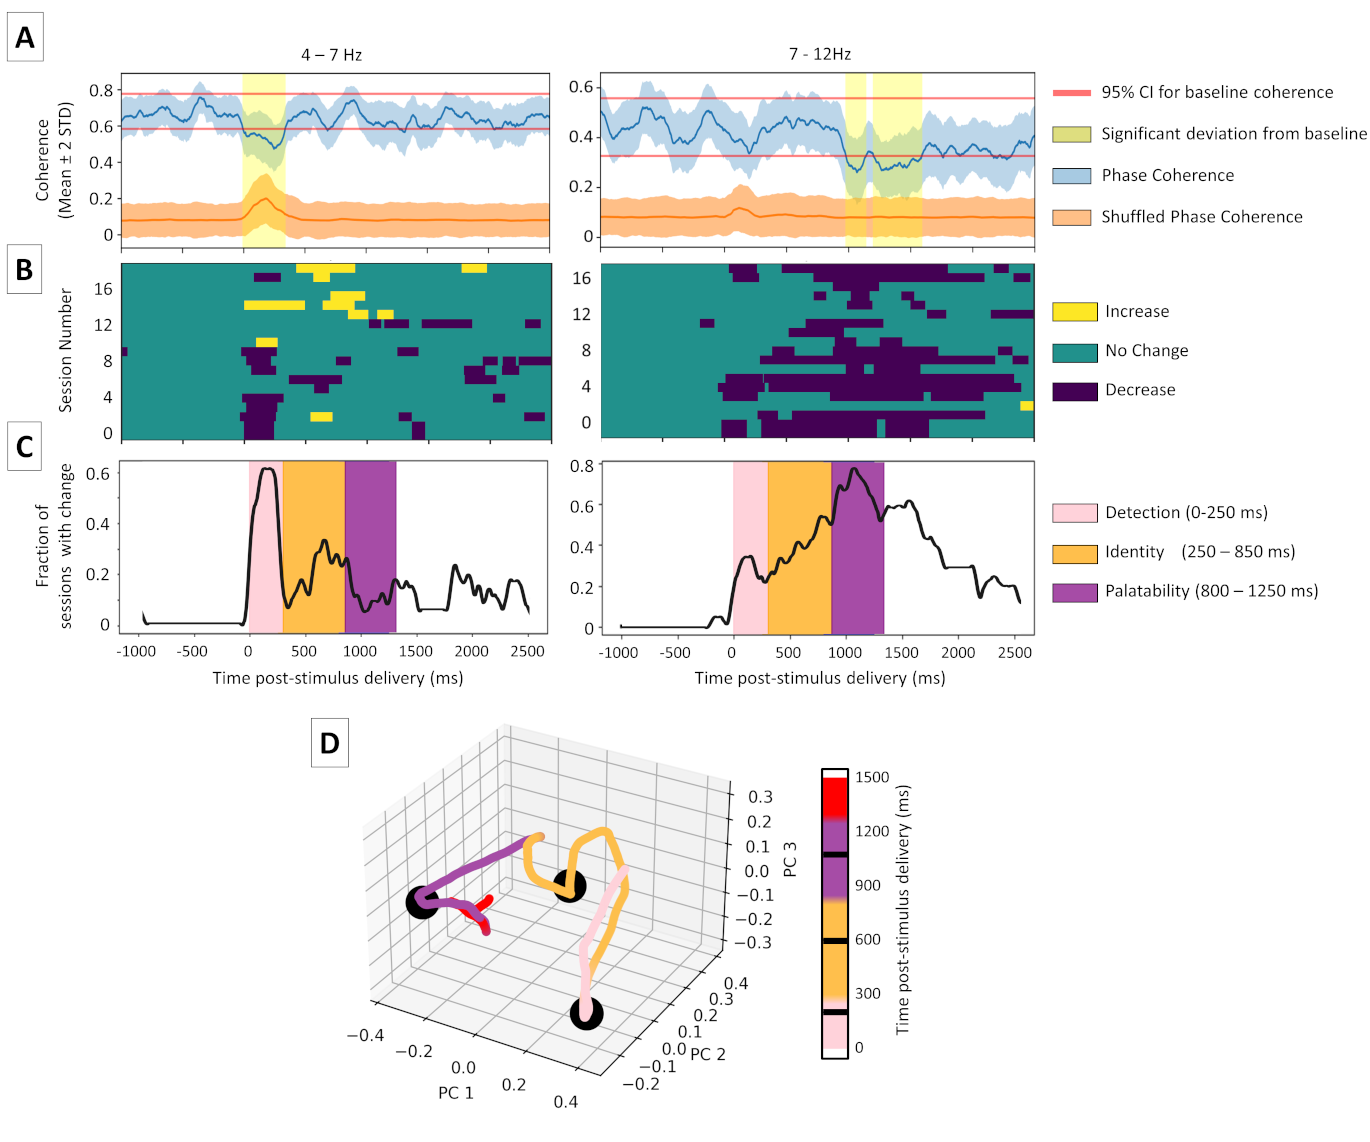
\includegraphics[width=\linewidth]{mahmood_22_figures/fig8-0.png}
\caption{\textbf{BLA-GC LFP phase coherence shows epoch-locked dynamics. (A)} Representative examples of phase coherence in the 4-7 Hz $\theta$, left) and 7-12 Hz $\mu$, right) bands. Red lines denote the 95\% confidence intervals determined by baseline coherence (-750 to -250 ms relative to stimulus delivery), and the yellow shading marks timepoints at which mean coherence changed significantly from that baseline. \textbf{(B)} Timepoints and directionality of changes in phase coherence relative to baseline for all sessions. While changes in the 4-7 Hz band show both increases and decreases (note that the most prominent changes from baseline, which are found in the earliest aspects of the responses, mostly consist of reductions of coherence), changes in the 7-12 Hz band consist entirely of decreases in coherence. \textbf{(C)} The fraction of recordings in which phase coherence deviated from baseline. Bands correspond to those of the plots above them. Note that the timepoints of changes in coherence relative to baseline match strongly with timings of the “canonical” taste epochs (noted with overlain shading). \textbf{(D)} PCA projection of changes in phase coherence (as in panel C) for 4-100Hz. Black circles indicate “corners” in the trajectory, the timings of which roughly correspond to each epoch (black ticks marks in colorbar). Colors indicate durations of epochs as in (C).}
\label{fig:wrapfig}
\end{figure}

To aggregate these results across the entire dataset, we calculated the fraction of recordings in which coherence diverged significantly from baseline at each time point across the evoked response (Fig. 3.8C). These results confirmed the representativeness of the examples above, showing that 4-7Hz coherence tends to be modulated early in the response, and that 7-12Hz coherence modulation comes on later in the response. While we have no specific explanation for why “theta” coherence highlights an earlier epoch and “mu” a different epoch, what is clear is that phase coherence illuminates the fact that BLA-GC coupling is modulated by epoch, as predicted.

To further illustrate the epoch-specificity of BLA-GC functional connectivity, we subjected deviations of coherence from baseline across a broad range of frequency ranges (4-7, 7-12, 12-30, 30-70, and 70-100Hz) to dimensionality reduction. In all bands we observed decrements in coherence, albeit with distinct temporal profiles (data for higher bands not shown). When we projected these timeseries of coherence deviation onto 3 principal components (Fig. 3.8D), the epoch-specific nature of BLA-GC coupling came into focus: the timing of sudden “turning points” in the trajectory, which are highlighted in Fig. 3.8D using black circles, roughly correspond to the center points of the canonical epochs. Collectively, these data strongly recapitulate the epoch-wise nature of taste processing that has been recognized in GC and BLA spiking data, demonstrating that BLA-GC functional connectivity is not static, and that BLA activity is explicitly tied to previously-described GC dynamics (\cite{lin2021a}).

\subsection{BLA and GC ensembles undergo coupled state transitions}
The structured dynamics of BLA-GC phase coherence suggests not only that BLA and GC population activity is coordinated, but that this coordination is modulated according to the unfolding taste response. It further suggests that the trial-to-trial variability in amygdala-cortical dynamics might be coupled, providing indirect evidence for our riskiest hypothesis --- that the sudden, behaviorally-relevant transitions between ensemble firing-rate states (transitions that are a reliable facet of GC ensemble taste activity and that occur at different latencies in different trials) might be a distributed network phenomenon, coupled across BLA-GC ensembles. Such nonlinear coupling would suggest that BLA and GC behave as a distributed, yet single (putatively attractor) network, processing tastes in a unified manner in real-time.

The analyses described in the above sections fall short of truly testing this hypothesis. In fact, they are strictly limited in their interpretability in this regard, specifically because population spiking changes in GC are quite sudden and the latencies of these transitions vary by hundreds of milliseconds from trial to trial (\cite{jones2006a,sadacca2016a}); these two properties of ensemble transitions ensure that any ability to evaluate their coupling will be essentially lost in across-trial averaging and obscured in moving-window analyses. Only through direct, single-trial analyses of the transitions themselves can we hope to evaluate BLA-GC coupling of such phenomena. 

\begin{figure}
\centering
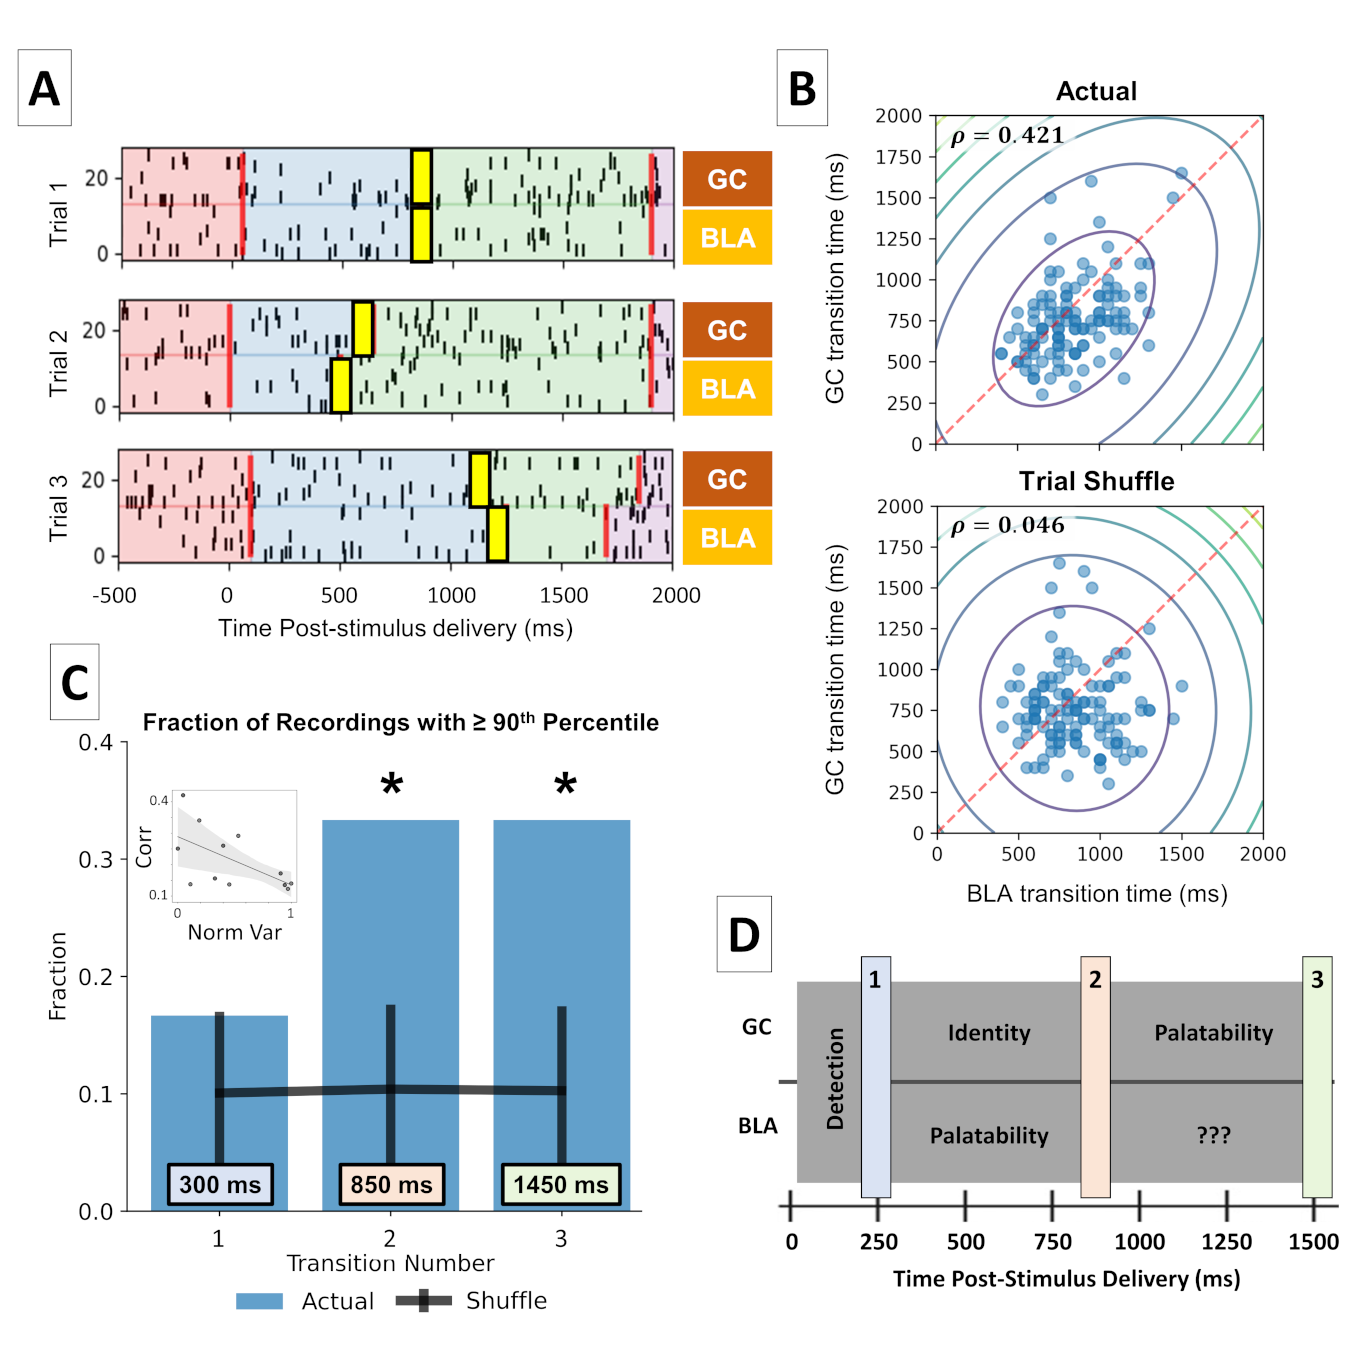
\includegraphics[width=0.9\linewidth]{mahmood_22_figures/fig9-0.png}
\caption{\textbf{BLA and GC population evoked responses involve coordinated state transitions. (A)} Three representative trials highlighting the co-variance of Transition 2 between BLA and GC. Transition 2 is highlighted with thick yellow lines. \textbf{(B)} The inferred times of GC state transitions plotted against those inferred for the simultaneously recorded BLA population for each trial of a representative transition; the scatterplot is overlain with contours of a 2D gaussian around the data cloud. The top plot shows actual data; the bottom, trial-shuffled data. $\rho$ = Spearman’s Correlation Coefficient \textbf{(C)} The fraction of datasets showing significant correlations for each transition (* : p\(<\)0.05). Blue bars represent the value in the actual data, and black lines indicate mean ± STD for fraction expected from random data. Only the fraction for Transitions 2 and 3 reached statistical significance. Colored boxes show average latency for each transition (post-stimulus delivery). \underline{Inset}: The variance (uncertainty) of transition latency distribution is significantly related to the correlation strength between BLA and GC transitions. Scatterplot shows correlation strength vs. normalized variance of inferred transition posterior distribution \textbf{(D)} The timings of the inferred transitions matches well with the canonical epoch-onset times. Transitions 2 and 3 bookend the palatability epoch in GC (figure adapted from \cite{fontanini2009a}).}
\label{fig:wrapfig}
\end{figure}

Given the novelty of this direct examination of inter-regional correlation of transition times, we first performed pilot analyses in which we divided datasets of simultaneously-recorded GC neurons into halves, separately applied changepoint inference to each half-population, and correlated the latency of each transition between the two fits. We observed statistically significant correlations for \(>\)80\% of our datasets and for each transition (n=11 recordings; data not shown), confirming that our correlation measure is a robust metric for determining transition coupling between ensembles (note that even these correlations were not significant for all datasets, and did not reach rho=1.0 for reasons discussed below, also see Methods). 
We then brought this analysis to bear on simultaneously recorded BLA and GC ensembles, independently estimating transition times in each, and then testing whether the latency of the 1st GC transition was correlated with the latency of the 1st BLA transition, etc. The results of this test, which are summarized in Fig. 3.9, demonstrate that certain transition times in BLA and GC ensembles are indeed robustly coordinated. Fig. 3.9A presents one representative set of spike-trains, showing inferred changepoints for a pair of simultaneously-recorded BLA and GC ensembles, and clearly revealing the close apposition of these transitions. Fig. 3.9B (top panel) shows a scatterplot of independently calculated latencies of the 2nd transition (the behaviorally-relevant transition into palatability-related firing in GC; \cite{sadacca2016a,mukherjee2019a}) from each of the trials for a representative session; the bottom panel of Fig. 3.9B shows the scatterplot that would be expected by chance (produced after randomly shuffling a set of changepoint latencies between trials for the same dataset). The significant covariance between the GC and BLA changepoints in the top panels is lost with trial-shuffling, proving that this transition alignment between the two regions is a within-trial phenomenon.

We statistically evaluated the strength of this BLA-GC transition coupling across the entire dataset by calculating the fraction of transitions that exceeded the 90th percentile of correlation strength relative to their respective trial-shuffled correlations (“strongly correlated” transitions), and statistically comparing this number to the fraction of strong correlations expected by chance for a similar sized dataset. This analysis revealed that the fraction of strongly correlated BLA and GC transition times in our data were significantly higher than those expected by chance, but only for the transitions into and out of the GC palatability-related state (Fig 9C; Percentiles=99.56 and 99.64, p=4.05x10$^{-3}$ and 3.65x10$^{-3}$ for transitions 2 and 3 respectively, Bonferroni-corrected alpha=0.05/3=16.67x10$^{-3}$, Shuffle test with Bonferroni’s correction, n = 18 recordings across 6 animals, see Methods). 

Note that this evidence of significant coupling --- the fact that the cloud of dots in the top panel of Fig. 3.9B is elongated --- is observed despite the relatively small ensembles of BLA neurons isolable in awake rats. It is quite likely that a good deal of the noise visible in this panel reflects unavoidable noise in the estimation of transition time (see Methods). To test this suspicion, we calculated the relationship between the amount of uncertainty in the model’s estimation of transition time (i.e., the summed average variance of inferred transition distributions) and the strength of correlation between GC-BLA transitions. As suspected, we found a significantly negative relationship between the two variables (Fig. 3.9C inset; slope=-2.3, r-squared=0.352, p=0.021, One-tailed Wald Test for regression slope), a result consistent with the suggestion that uncertainty in the inference “blurs” the correlation between transitions. The strength of coordination between BLA and GC transitions is, thus, likely even stronger than that estimated here.

Note, however, that only transitions in and out of the state that has been previously shown to be related to the reaching of consumption decisions (\cite{sadacca2016a}), i.e. transitions that signaled the onset and offset of the “palatability” state in GC (schematic shown in Fig. 3.9D), were coupled across the BLA-GC network; transitions from the GC Detection state into GC Identity states were not. This result dovetails nicely both with classic thinking about the specific role of BLA in emotional processing (Yamamoto, 2008; Baxter and Croxson, 2012) and with recent work from the lab which shows that optogenetic perturbation of the BLA$\rightarrow$GC projection primarily affects GC processing during the palatability epoch in GC (\cite{lin2021a}). While BLA activity during the late epoch (“???” in Fig. 3.9D) has hitherto not been explored, the strong BLA-GC coupling during that time period recommends further investigation into processing performed by BLA during that time period. Together, these results suggest that the “role” of BLA-GC communication likely changes between epochs, and even may only be important during the GC palatability epoch.

\subsection{Modelling coupled state-transitions with state-specific coherence}
Together, the above results fill in a picture of BLA and GC as processing tastes as a single distributed unit, with significant (above-chance) cross-coherence punctuated by coupled state transitions across which the coherence drops in certain frequency ranges (a change indicative of intense processing). From a dynamical systems perspective, this phenomenology makes sense: “instantaneous” coherence will often be state-specific within a system in which state transitions are synchronized across brain regions; for just one example, brain regions collectively transition between different states of sleep; \cite{stitt2017a}. We would argue, in fact, that it is common for distributed networks of interconnected neurons to perform coupled transitions between states, some of which demonstrate decreases in LFP phase coherence.

\begin{figure}
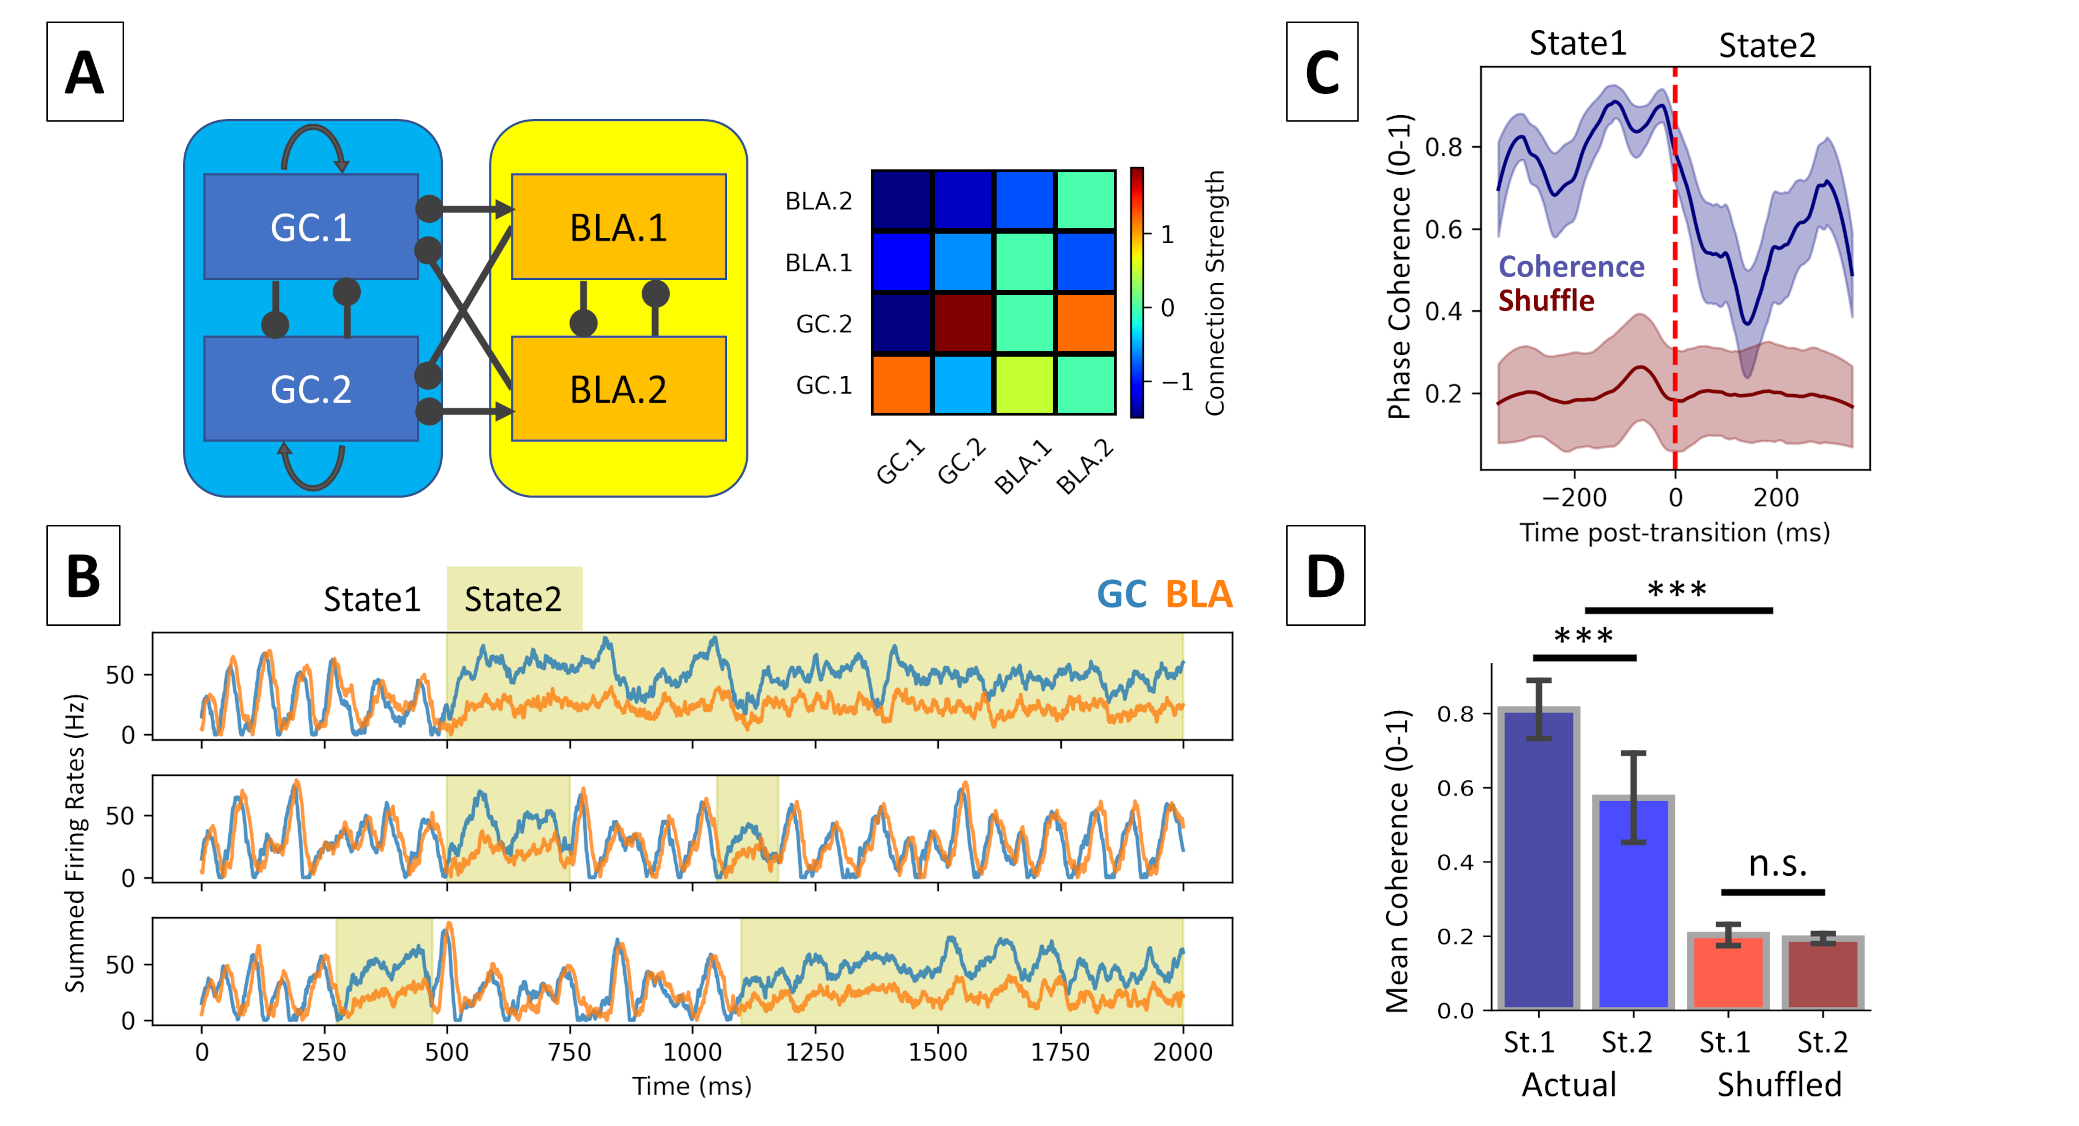
\includegraphics[width=\linewidth]{mahmood_22_figures/fig10-0.png}
\caption{\textbf{Coordinated state transitions and state-specific coherence in a coupled network model. (A)} Network of 4 inter-connected "subpopulations" which represent parts of GC and BLA \textbf{(B)} Example "trials" showing activity of the network. Activity from both units in each region is summed as an analog of LFP. Highlighted regions marks time periods the system spends in the less coherent state (State 2). Note that both states have finite durations. \textbf{(C)} Inter-trial phase coherence calculated on time windows 350ms before and after transition from State 1 $\rightarrow$ State 2 (more$\rightarrow$less coherent state; mean ± std). \textbf{(D)} Average coherence during each state (mean ± std; St.1 = State 1, St.2 = State 2, *** = p\(<\)0.001).}
\label{fig:wrapfig}
\end{figure}

We tested this contention by constructing a simple network model. Briefly, the network was comprised of firing-rate units which can be taken to roughly represent interconnected subpopulations of BLA and GC neurons (Fig. 3.10A; the right panel shows the connection strengths between subpopulations). When challenged with a moderate amount of input delivered to both “regions” (simulating either noise or taste stimulation, which initially arrives at BLA and GC via distinct paths; see \cite{gal-ben-ari2012a}), the network enters a mode in which it switches between a “more coherent” state characterized by strong oscillations, and a “less coherent” state where clear oscillations are disrupted (a switch that necessarily changes functional connectivity). Fig. 3.10B presents the summed firing rates of simulated BLA and GC units across 3 “trials,” in which the network can be seen to collectively transition between the states, one of which is clearly endowed with higher cross-coherence (State 1) than the other (State 2).
Fig. 3.10C provides a specific analysis of these appearances, revealing that coherence indeed decreases following the transition into the less oscillatory state (State 2). In neither state, however, does this cross-coherence decline to baseline levels --- the populations never fully disconnect (Fig 10C and 10D, 2-Way ANOVA with State and Dataset [Actual vs Shuffle] as factors, State : F(1) = 184, p=0.001; Dataset : F(3) = 184, p=0.001; State*Dataset : F(3) = 233, p=0.001; Tukey’s HSD post-hoc tests, Actual St.1 vs St.2 : T = 42.7, p = 0.001; Shuffle St.1 vs St.2 : T = 1.74, p = 0.302). And while this network is admittedly simple (a fact that no doubt explains the simple, randomly-timed "back and forth" between two states), it is not the only way that such a model can be constructed: other versions can allow each region to intrinsically oscillate at different resonant frequencies, for instance, where such frequencies would inevitably be expressed to differing degrees in different states. The important point is that this variant of the model would, like many such variants (and the real networks recorded for this study), progress through state transitions in a unified manner, and that phase coherence would be lower following certain transitions. While our investigation of the model is limited to recapitulating the state-specific changes in coherence we see in our data, this recapitulation further highlights the aptness of such “attractor models” for explaining activity in GC and BLA, and therefore being good candidates for theoretical investigation to generate predictions about the system to be tested in future experimental work (also see Discussion).

Ultimately, these simulations demonstrate that a multi-region network can undergo collective, coupled state transitions while having variable functional connectivity during each state. We suggest that the amygdala-cortical system is just such a network.

\section{Discussion}
Much of the research that has explored how brain regions work together (\cite{markov2014a,grabska-barwi2017a,yates2017a,glaser2018a}) makes two broad assumptions: 1) neural responses are identical (save for noise) across repeated stimulus presentations; and 2) neural dynamics evolve on slow timescales (hundreds of milliseconds, or even seconds). These assumptions fail in many cases (\cite{gat1997a,sugase1999a,latimer2015a,jones2007a}), including the present study. In such cases, examination of coupling requires methodologies that can parse sharper changes in neural activity and account for trial-to-trial variability.

In the context of taste processing, gustatory cortex (GC) and basolateral amygdala (BLA) form strong candidates for coupling. Both are involved in driving taste-related behavior --- perturbations of either results in similar behavioral changes (\cite{lovaglio2010a,lin2011a,lin2018a}), perturbation of BLA changes GC response dynamics (\cite{piette2012a}), and BLA-GC connectivity is important for taste learning (\cite{lin2012a}). Furthermore, taste-evoked activity of single-neurons in the two structures (\cite{fontanini2009a,sadacca2012a}) undergoes changes (and encoded information) at the same time points. 

These facts motivate the current study but stop short of actually testing the hypothesis that BLA and GC transition synchronously. Hitherto, the most direct test of BLA-GC coupling has involved acute optogenetic perturbations of BLA$\rightarrow$GC axonal projections (\cite{lin2021a}). This perturbation decreased GC ensemble coherence during the transition to palatability coding, and reduced palatability-relatedness of single-neuron firing following this transition. Brief, bilateral optogenetic perturbation of GC neurons themselves, meanwhile, delivered before or during this transition to palatability coding (\cite{mukherjee2019a}), delayed the gaping response of rats to bitter quinine until after the perturbation was removed; hence, while this GC perturbation hindered planning and execution of the taste motor response, it is likely that the remainder of the circuit maintained output-relevant information, enabling a rebound from the perturbation. 

Results of the above studies --- the fact that some palatability-related information in GC survives silencing of BLA$\rightarrow$GC axons, and the fact that gaping quickly recovers after GC perturbation-in conjunction with the results from the current study, suggest that while BLA and GC are strongly coordinated, they are only parts of an even larger network. This conclusion is further bolstered by work showing: 1) that other brain regions show response dynamics similar to BLA and GC (lateral hypothalamus : \cite{li2013a}; and parabrachial nucleus of the pons : \cite{baez-santiago2016a}); and 2) that while palatability responses in GC show a gradient of hedonic values, those in BLA are largely binary (good vs. bad, \cite{fontanini2009a,sadacca2012a}). Clearly, there are additional regions (perhaps the lateral hypothalamus) that process palatability information in parallel to BLA to produce the more nuanced coding seen in GC. 

In this context, our results are also consistent with those showing that distributed nodes in tightly-coupled systems can produce non-identical coding during stimulus processing, and encode “redundant” information to varying degrees (\cite{siegel2015a,brincat2018a,lara2018a,saravani2019a}). This is not truly surprising: complex systems tend to couple on multiple time-scales; just as one unit of such a system might increase its spiking while another is silent, and vice-versa (Fig. 3.6A), one’s firing might reflect palatability at one time point, and then the other do so afterward. The fact that palatability-relatedness moves from BLA to GC might simply reflect a single cycle of an oscillation.

The advance offered in this study has to do with the subtlety of the predicted coupling, which rendered previously-used methodologies for investigating that coupling insufficient. Specifically, we predicted that (trial-specific) moments of ensemble state transitions in GC and BLA would be synchronized. This hypothesis could not be tested using analyses that fail to account for dynamics of functional connectivity, collapse data over large time-scales (e.g. whole trials), or assume that all trials are dynamically identical. In the current context, such analyses provide misleading information: both the spike-count correlation and the LFP-phase coherence analyses show BLA and GC to be significantly coordinated but fail to give us any information about temporal dynamics; meanwhile, changes in BLA-GC inter-trial phase coherence (which is de rigeur for characterizing inter-regional coupling, see \cite{engel2020a,kramer2020a,zareian2020a,zielinski2019a}) reveal only state-specific reductions in coupling (Fig. 3.8).

Such state-specific changes in coherence have been seen in transitions between sleep states (\cite{stitt2017a}), and between attentive and inattentive states (\cite{siegel2008a}). While the states in evoked activity described in this paper are more fleeting than the much longer brain states studied by \cite{stitt2017a,siegel2008a}, in each case changes in phase coherence mark changes in brain states. Specifically, reductions in coherence such as we observe here have been shown to be associated with intense processing (\cite{supp2011a}), whereas increases in coherence are associated with cognitive impairments (\cite{martinet2017a,arbab2018a}). Such low correlations in activity are entirely compatible with strong coupling (\cite{schneidman2006a}). Particularly given the fact that BLA-GC phase coherence always stays well above chance levels, it is safe to say that this observation of decreased coherence does not mean that GC and BLA are becoming “decoupled” at any time point. 

Again, had we stopped our analysis at phase coherence, we would have reached the wrong conclusion about amygdala-cortical coupling during taste processing; only the novel transition coordination analysis (which accounts for both dynamics over the course of the trial and variability across the trials) allowed us to directly test the risky hypothesis that taste processing is characterized by sudden ensemble state transitions shared across BLA and GC. Our successful test of this hypothesis strongly corroborates the results of causal studies showing that wholesale inhibition of BLA (\cite{piette2012a}) and precise perturbation of the BLA$\rightarrow$GC axonal projection (\cite{lin2021a}) specifically perturb processing during --- and the transition to --- the palatability-related (late) epoch of GC taste coding. This further underscores the limitations of more canonical communication measures with regard to the theories that they are able to test, and provides further evidence for the dynamic nature of the BLA-GC interaction.

Together, these results suggest that taste responses observed in BLA and GC are poorly described by feedforward/hierarchical (\cite{parras2017a,glaser2018a,heidari-gorji2021a}) models, and better described as working in a joint fashion. Our finding of coordinated state-transitions is appealingly (if speculatively) explained in terms of collective attractor states (\cite{miller2010a,litwin-kumar2012a,camera2019a,recanatesi2022a}). Such models require strong, bidirectional connectivity that is observed throughout the taste circuit (Bielavska and Roldan, 1996; McDonald, 1998; Shi and Cassell, 1998), and predict/recapitulate the sharp state transitions that have been reported in GC (\cite{jones2007a,sadacca2016a}), BLA (this study), and other brain regions (\cite{seidemann1996a,gat1997a,sugase1999a,latimer2015a}). Another attractive aspect of such a theory is the fact that “noise”, rather than being a nuisance variable, serves as the force driving state transitions, allowing robust performance in noisy conditions (\cite{miller2013a}) and explaining the large variability observed in evoked neural and behavioral responses on a trial-by-trial basis (\cite{kisley1999a,carandini2004a,jones2007a,kotekal2020a,peixoto2021a}). Given the ubiquity of “noise” in biological systems (\cite{shadlen1994a,shadlen1998a,miller2010a}), it seems likely that valid mechanisms of function will be those that have this property. 

Of course, causal confirmation of this theory waits upon evidence that the two structures influence one another recurrently --- i.e. studies investigating the role of the GC$\rightarrow$BLA (“reverse”) projection in taste processing. While the GC$\rightarrow$BLA projection has been shown to be important for taste-related learning, (\cite{lavi2018a,kayyal2019a}), it’s role in generating passive taste responses is yet to be elucidated. If recurrent circuitry plays a role in taste processing, perturbation of the GC$\rightarrow$BLA projection should change not only activity in BLA but also the “source” activity in GC, reflecting the fact that the circuit processes information in a loop fashion. Such an outcome would further drive home the value of moving away from “feedforward” biases in the study of taste processing. 

Ultimately, a nuanced understanding of inter-region communication, and of how this communication is important for generating behavioral output, will require that we appreciate the sorts of nonlinearities and variability examined here --- that we do not smooth out potentially important sudden ensemble changes in real-time ensemble activity. The current study furthers our trial-specific understanding of neural activity and will hopefully drive further questions regarding the role of reciprocal connectivity and meta-stable dynamics in sensory processing.

\begin{singlespace}
\printbibliography[title={References}]
\end{singlespace}

\end{refsection}